\documentclass[12pt,twoside]{report}
\usepackage[utf8]{inputenc}
\usepackage{graphicx}
\usepackage{hyperref}
\usepackage{wrapfig}
\hypersetup{pdftex,colorlinks=true,allcolors=black}
\usepackage{hypcap}
\graphicspath{ {images/} }
\usepackage{amsfonts}
\usepackage{amsmath}
\usepackage{amssymb}
\usepackage{subfig}
\usepackage{epsfig}
\usepackage{physics}
\usepackage{color}
\usepackage[a4paper,width=150mm,top=35mm,bottom=35mm,bindingoffset=6mm]{geometry}
\usepackage{wrapfig}
\usepackage{eurosym}
\usepackage{titlesec, blindtext}
\usepackage[numbers]{natbib}
\usepackage{epigraph}
\usepackage{wrapfig}
\pagenumbering{roman}
\usepackage{fancyhdr}
\usepackage[rightcaption]{sidecap}



\begin{document}
	\begin{center}
		
		\Large \textbf{Optical Properties of Active and Passive Photonic Resonators}
		
	\end{center}
\begin{center}
	\begin{figure}[h]
	\centering
	
\includegraphics[width=5cm,height=7cm,keepaspectratio]{universitye.jpg}\\
	\end{figure}
\end{center}
	\begin{center}
		\emph{\large by}\\
		
		\Large \textbf{AHMAD BILAL}\\
		\Large CIIT/FA15-BPH-019/ISB\\
		\vfill
		\Large BS Thesis\\
		\Large In\\
		\Large Physics
	\end{center}
	\vfill
	\begin{center}
		\Large \textbf{COMSATS University Islamabad}\\
		\Large Islamabad - Pakistan
	\end{center}
	
	\begin{center}
		 Spring, 2019
	\end{center}
	\newpage
	\noindent
	\begin{wrapfigure}{l}{0.12\textwidth}
		\centering
		
\includegraphics[width=1\linewidth]{university.jpg}
	\end{wrapfigure}
	\begin{center}
	{\Large{ \textbf{COMSATS University Islamabad}}}
	\end{center}
	
	\vspace{0.2 in}
	
	\begin{center}
		{\Large {Optical Properties of Active and Passive Photonic Resonators
		} }
	\end{center}
	\vspace{0.5 in}
	
	\begin{center}
	{A Thesis Presented to}
	\end{center}
	\vspace{0.2 in}
	\begin{center}
		{\Large {\textbf{COMSATS University Islamabad}} }
	\end{center}
	\vspace{0.5 in}
	\begin{center}
		{In partial fulfillment }
	\end{center}

	\begin{center}
		{of the requirement for the degree of}
	\end{center}
	
	\vspace{0.5 in}
	
	\begin{center}
		{\Large {\textbf{Bachelor of Science in Physics}} }
	\end{center}
	
	\vspace{0.5 in}
	\begin{center}
		{by }
	\end{center}
	\begin{center}
		{\large {Ahmad Bilal\\[0pt]
				CIIT/FA15-BPH-019/ISB\\[0pt]
		}}
	\end{center}
	\vspace{0.5 in}
	\begin{center}
		Spring, 2019
	\end{center}
	\newpage
	\begin{center}
{\Large {Optical Properties of Active and Passive Photonic Resonators}\\[0pt]
		\noindent\rule{18cm}{3pt}} \\
\end{center}
\vspace{0.2 in} 
		An Under Graduate Thesis submitted to the Department of Physics as partial fulfillment of the requirement for the award of Degree of BS (Physics). 
\vspace{0.5 in}
\begin{center}
	\begin{tabular}{ | c| c | }
			\hline
			Name &  Registration Number \\
			\hline
		Ahmad Bilal & CIIT/FA15-BPH-019/ISB \\ 
			\hline
	\end{tabular}
\end{center}
	\vspace{3 in}
	\textbf {Supervisor:}\\
	Dr. Ahmer Naweed,\\
	Associate Professor,\\
	Department of Physics,\\
	COMSATS University Islamabad (CUI).\\
	\newpage
	
	\begin{center}
		\textbf{\Large{Final Approval}}
		\noindent\rule{15cm}{1pt} \\

		This thesis titled\\
		\vspace{0.5cm}
{\Large \textbf {Optical Properties of Active and Passive Photonic Resonators}}\\
\vspace{0.3cm}
By\\
\emph{Ahmad Bilal}\\
\emph{CIIT/FA15-BPH-019/ISB}\\
\vspace{0.1 in}
Has been approved\\
\vspace{0.1 in}
For the COMSATS University Islamabad\\
\end{center}
\vspace{0.5cm}
External Examiner: \noindent\rule{8cm}{0.4pt}\\
\begin{center}
	Dr. Muhammad Khalid Khan\\
	Professor, Dept. of Physics\\
	Quaid-i-Azam University Islamabad\\
\end{center}
Supervisor: \hspace{1.35cm}\noindent\rule{8cm}{0.4pt}\\
\begin{center}
	Dr. Ahmer Naweed\\
	Associate Professor, Dept. of Physics\\
	COMSATS University Islamabad\\
\end{center}
\vspace{0.5cm}
HoD: \hspace{2.5cm}\noindent\rule{8cm}{0.4pt}\\
\begin{center}
	Dr. Sajid Qamar\\
	Professor, Dept. of Physics\\
	COMSATS University Islamabad
\end{center}
	\newpage
	\begin{center}
		\textbf{\Large{Declaration}}
		\end{center}
I, \underline{\textbf{Ahmad Bilal} (CIIT/FA15-BPH-019/ISB)} hereby declare that this project
neither as a whole nor as a part there of has been copied out from any source. It is
further declared that I have developed this thesis and the accompanied report entirely
on the basis of my personal efforts made under the sincere guidance of my supervisor.
No portion of the work presented in this report has been submitted in support of any
other degree of qualification of this or any other University or Institute of learning, if
found I shall stand responsible.  \\\\\\\\\\
Date: \underline{}  \\\\\\
\begin{flushright}

	\noindent\rule{4cm}{0.4pt} \\  Ahmad Bilal \\   CIIT/FA15-BPH-019/ISB 

\end{flushright}

	
\newpage
\begin{center}
\textbf{\Large{Certificate}}\\
\end{center}
It is certified that \underline{Ahmad Bilal (Registration No. CIIT/FA15-BPH-019/ISB)} has carried out all the work related to this thesis under my supervision at the Department of Physics, COMSATS University Islamabad and the work fulfills the requirement for award of BS degree. \\\\\\
Date: \noindent\rule{3cm}{0.4pt}
\vspace{2.5cm}
\begin{flushright}
Supervisor: \\
\noindent\rule{4cm}{0.4pt}\\
Dr. Ahmer Naweed \\
Associate Professor\\ Department of Physics\\
\end{flushright}
\vspace{3cm}
Head of Department: \\
\noindent\rule{4cm}{0.4pt}\\
Dr. Sajid Qamar \\
Department of Physics
\newpage	


\chapter*{{\Large Dedication}}
\normalfont \large This thesis is dedicated to my mother who brought me up all by herself, motivated me to always pursue my dreams, and made me the gentleman I am today.
\addcontentsline{toc}{chapter}{Dedication}


\chapter*{{\Large Abstract}}
\paragraph{\normalfont Since long, electronic integrated circuits has dominated our modern technology. Now with the dawn of photonics, which is basically using integrated circuits made up using optics, it is not far that our modern technology takes a new toll and slide into a new generation of digital devices. Photonics is the technology of generating and harnessing light and other forms of radiant energy whose quantum unit is a photon.}  

\paragraph{\normalfont In this project, we have investigated the optical characteristics of coupled ring resonators, which may be either active (containing a gain element) or passive. In the case of passive coupled resonators, intrinsic and coupling losses affect the circulation, transmission, and dispersion of an input optical pulse. However, for active coupled resonators, gain excitation may be used to compensate for the losses. This alters the spectral and dispersive properties of the coupled-resonator system owing to the enhancement of the quality factor of the system. We demonstrated gain tunable all-optical analogs of Electromagnetically Induced Transparency (EIT) and Electromagnetically Induced Absorption (EIA). This allows us to precisely control the subluminal and superluminal group velocities of light pulses. Furthermore, we demonstrate the gain-mediated reversible transition between the sub and superluminal dispersion regimes.}

\paragraph{\normalfont The optimized coupled resonators enable continuous tuning of sub and superluminal group velocities. Furthermore, owing to gain manipulation, the transmission and light confinement duration may also be precisely tuned. These features make the coupled resonator system attractive for future applications in optical and quantum information science.}

\addcontentsline{toc}{chapter}{Abstract}

\newpage
\pagestyle{empty}
\phantomsection
\begin{flushright}
\textit{\small{Indeed, in the creation of the heavens,\\ and the earth and the alternation of\\ the night and the day, are signs for\\ those of understanding.\\ The Nobel Quran [3:190]}}
\end{flushright}
\noindent\rule{15cm}{1pt}
\begin{flushleft}
\textbf{\Large{Ackowledgement}}
\end{flushleft}
\noindent\rule{15cm}{1pt} 
\addcontentsline{toc}{chapter}{Acknowledgement}
\paragraph{ \normalfont In the name of Allah, who is the most beneficent and merciful. I would start off this extensive documentation with a quote from Carl Sagan, one of the greatest science educator ever, who created enough enthusiasm and curiosity in me to pursue my career in Physics. He said, \textit{“Somewhere, something incredible is waiting to be known".} This is one of the reasons I chose to be a student of physics, it inspires me to search for the unknown clues that are hidden in the very fabric of reality. Physics gave mankind the power to dominate their world and use the best of nature for their benefit.}
\subparagraph{ \normalfont Since childhood, I had always been fascinated by computers and gadgets. Having the background of engineers in my family, I almost ended up joining computer engineering in High School. But the curiosity inside me had made me a stargazer. So I had questions about how do they get where they are, and what are they made of? These questions were those which made me switch my field to Physics which is a science of never-ending curiosity. In this process, a lot of people are included some directly and some indirectly, most of which is my family, because their never-ending support had made me chase my dreams.}
\subparagraph{ \normalfont So, to start off, I would personally like to thank my supervisor in this BS project, Dr. Ahmer Naweed, whose outstanding supervision and guidance had helped me through thick and thin to complete this project and he also kept me motivated enough to continue my research in the field of photonics. I would like to thank my batch counselor Dr. A. H. Mujtaba, whose support and teachings made us all work harder and harder for the progression of science. Also, thanks to Ms. Zarqa Zahid for recommending me to Dr. A. Naweed. I would like to thank Dr. Siraj-ul-Islam Ahmad for motivating me and providing me help in computation related issues that I have encountered during this thesis. Also, I would like to thank all my peers and my batch mates of Fall 15, because the support and love I get from them is immeasurable. Then again I would like to thank my family and especially my mother, who never asked me about my grades and have always said, “if you love what you are studying, only then you can achieve true learning."}
\subparagraph*{ \normalfont	In the end, it is important to know that knowledge is a never-ending process, and Physics is such a beautiful field that every time I learn a new concept about the universe and its principles, it feels like I have been born again.} 
\begin{flushleft}
\noindent\rule{5cm}{0.5pt}\\
\textbf{\small Ahmad B. Yousafzai}\\
\textbf{\small Islamabad, May 2019}
\end{flushleft}


\begin{scriptsize}
%\large 
\small \tableofcontents
\end{scriptsize}
\small \listoffigures
\newpage
\pagenumbering{arabic}
\fancyhead[RO,LE]{}
\fancyfoot[CO,CE]{\small OPTICAL PROPERTIES OF ACTIVE AND PASSIVE RESONATORS}
\fancyfoot[LE,RO]{\thepage}
\renewcommand{\footrulewidth}{0.5pt}

\pagestyle{fancy}

\chapter{Introduction}
\normalfont \large Since the dawn of modern technology, the integrated circuits on which today our every electronic device operates, we have progressed a lot in developing faster and smaller computing devices. Decades have passed since electric circuits became integrated on microchips, also called ICs. This technology has no pause but the field of optical research which generated a great amount of research progress raised to a new form of technology on which we can operate our computing circuits called Photonics. Now is the time that we integrate photonic crystals and photonic structures on circuits and make use of them in communication, signal processing, biochemical sensing, slow and fast light structures [1], optical filters, optical buffers [12-13], wavelength-division-multiplex (WDM)[5-8] and on-chip optical interconnects [8]. Every phenomenon mentioned here is made possible by confining light in a very small volume. micro resonators can be used to support the spectrum of optical modes with required polarization frequency and field patterns. These research phenomena will bring revolution to the digital technology, as we know today, with every hand-held device to corporate machines, all running on circuits made using photonic crystals and optical microresonators [9-11]. 
\subparagraph{\normalfont \large On a basic level, there are so far two settled components of light control and direction inside the volume of an optical microresonator. The rest is the ordinary system of Total Internal Reflection (TIR) and the presence of evanescent waves, where the directing medium must be optically denser, i.e., have a higher refractive index, than the encompassing one so as to accomplish light constrained. The second is the photonic bandgap (PBG) found in artificial optical media having a spatial periodicity in one, two, or three measurements, named photonic crystals (PC), which is a consequence of the phenomenon of Bragg reflection causing the arrangement of frequency bands where propagation of light is restricted by the destructive interference of field harmonics inside the crystal. Exceptionally bound optical modes can be accomplished in these bands when certain deformities are presented in the generally flawless intermittent crystals. With PC defect modes, the light can be found in a size similar to its wavelength $(\lambda/n)$, where $\lambda$ is the vacuum wavelength and $n$ is the medium refractive index.[11]}

\subparagraph{\normalfont \large These topics required a detailed study, which is what we are going to do in this Thesis. The scope of this thesis is not limited to the certain and most applicable type of optical resonator which is known as Whispering Gallery Resonators (WGR) [2], but we are going to extend this research on to different possible and quite promising arrangements and geometries of optical resonators known as Micro Ring Resonators (MRR) [5]. In Micro ring resonators we mainly focus on the ring-shaped optical wave-guides introducing coupling and different modes in a single and composite system of resonators. This will allow us to collectively measure and observe the combined effects of such resonators by studying their optical properties. Broad numerical and exploratory investigations have been committed towards the investigation of at least two coupled cavities, and a few significant applications have been illustrated, including upgraded spontaneous emission inferable from mode-density enhancement at the photonic band edge [16], enhancement of cavity quantum electrodynamics effects [17], realization of
quantum-optical Josephson interferometer [18], parametric oscillations in a triple microcavity
system [12], dual wavelength lasing [19], and realization of photodetectors for highperformance wavelength demultiplexing [14]. Coupling effects have been observed in detail and have made possible to observe effects like Electromagnetically Induced Transparency [20] and Electromagnetically Induced Absorption in coupled resonator systems which are called Coupled Resonator Induced Transparency and Coupled Resonator Induced Absorption [2].}
\subparagraph{\normalfont \large This document is divided into different sections by compiling the work of 1 year long BS final year project. First, we will increase the understanding of the reader of what interferometers, resonators, optical resonators, and micro ring resonators are. Then, their underlying physics and relating phenomenons that are followed by the regimes of these optical systems and what outcome could be achieved by using these optical systems and their applications in photonics. Then we will focus on the systems that we used in this research process and their basic physical explanations. After that, I will show you the results of what I have collected by modeling these systems in different conditions (parameters). This extensive documentation will be useful for anyone trying to get started in this field of research because it is written in such a manner that a newbie in the field of photonics can easily grasp the ideas and can learn from it. }

\section{Resonators}
\normalfont \large A resonator is a device that exhibits resonant behavior naturally (or artificially) on some resonant frequencies, that is, it oscillates at frequencies with higher amplitudes than others. These frequencies are called resonant frequencies. These oscillations can either be electromagnetic waves or mechanical waves as well. There are different uses of resonators, they can be used to filter some specific frequencies or can also be used to generate a specific frequency of the wave. A resonator in which the waves exists in hallow space is called a cavity resonator, which is used in electronics and radio signal processing, known as microwave cavities, to generate, transmit and receive electromagnetic signals. Acoustic cavity resonators, in which sound is produced by air vibrating in a cavity with one opening, are known as Helmholtz resonators.
\subsection{Principle}
The term resonator is most often used for a homogeneous object in which, vibrations travel as waves, at an approximately constant velocity, bouncing back and forth between the sides of the resonator. The material of the resonator, through which the waves flow, can be viewed as being made of millions of coupled moving parts (such as atoms). Therefore, they can have millions of resonant frequencies, although only a few may be used in practical resonators. The oppositely moving waves interfere with each other, and their resonant frequencies reinforce each other to create a pattern of standing waves in the resonator. If the distance between the sides is ${\displaystyle d\,}$, the length of a round trip is ${\displaystyle 2d\,}$. To cause resonance, the phase of a sinusoidal wave after a round trip must be equal to the initial phase so the waves self-reinforce. The condition for resonance in a resonator is that the round trip distance, ${\displaystyle 2d\,}$, is equal to an integer number of wavelengths ${\displaystyle \lambda \,}$ of the wave:

$${\displaystyle 2d=N\lambda ,\qquad \qquad N\in \{1,2,3,\dots \}}$$

If the velocity of a wave is ${\displaystyle c\,}$, the frequency is ${\displaystyle f=c/\lambda \,}$ so the resonant frequencies are:

$${\displaystyle f={\frac {Nc}{2d}}\qquad \qquad N\in \{1,2,3,\dots \}}$$

So the resonant frequencies of resonators, called normal modes, are equally spaced multiples (harmonics) of the lowest frequency called the fundamental frequency. The above analysis assumes the medium inside the resonator is homogeneous, so the waves travel at a constant speed, and that the shape of the resonator is rectilinear. If the resonator is inhomogeneous or has a nonrectilinear shape, like a circular drumhead or a cylindrical microwave cavity, the resonant frequencies may not occur at equally spaced multiples of the fundamental frequency. They are then called overtones instead of harmonics. There may be several such series of resonant frequencies in a single resonator, corresponding to different modes of vibration. [1]

\section{Optical Resonators}
An optical resonator, also known as an optical cavity, is usually composed of two highly reflecting mirror held in front of each other parallelly inside a vacuum so that the system exhibits resonant behavior which allows standing wave modes to exist with almost no loss. Thus optical resonator is a cavity with walls that are highly reflected for electromagnetic waves (i.e light).

\begin{figure}[h]
\centering
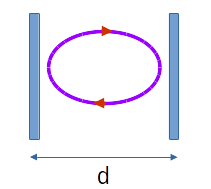
\includegraphics[scale=0.75]{optical_cavity.png}
\caption{Illustration of a basic optical cavity.}
\end{figure}

\section{Different Types of Optical Resonators}
\subsection{Fabry-Perot Resonator}
A system of two mirrors held parallel to each other and both having high reflectivity’s show a resonant behavior at some frequencies of the incident light. If both the mirrors have high reflectance, the incident light is still observed to pass through them without any decrease in the intensity and is detected, which occurs due to phenomenon’s similar to quantum tunneling effects [14].

\subsection{Gires-Tournois}
It is basically a lossless Fabry-Perot resonator which has a 100$\%$ reflecting rear mirror, that means it reflects 100$\%$ at all frequencies. Still, some resonant frequencies stay between the mirrors for a longer period of time and thus descript resonant behavior and lead to ultra slow group velocities. This simple device is known for storing spectral power of light which is reflected from it while modifying its phase. That is why it is sometimes referred to as a "phase only" filter.


\section{Micro Resonators}
Microresonators are a special type of resonators made from a different type of materials which exhibit optical properties while being fabricated on a chip [8]. These kinds of resonators are actually useful in observing the effects of optical resonators on a device.

\subsection{Different Geometeries}
There are many types of microresonators from which micro ring-resonators are very useful in making photonic devices and have a wide variety of application. Other kinds of resonators are also useful for different kind of applications and all have distinct optical properties based on their geometry. (See figure 1.2)
\begin{figure}[h]
\centering
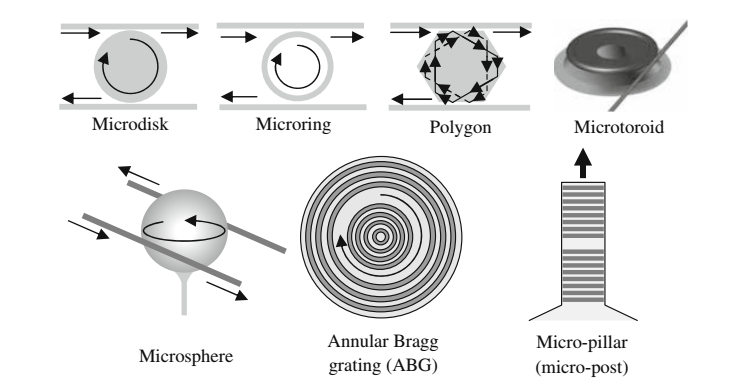
\includegraphics[width=1\textwidth]{microresonators_types.jpg}
\caption{Different geometries of microresonators.[15]}
\end{figure}


\section{Electromagnetically Induced Transparency and Absorption (EIT and EIA)}
Electromagnetically Induced Transparency (EIT) is a coherent optical nonlinearity which makes a medium transparent to some narrow bandwidth of frequencies which were otherwise opaque to the incident radiation. This window leads to slow light at resonant frequencies in an optical resonant system usually involving coupled system. This is observed due to the destructive quantum interference effects of the incident radiation in atomic levels [4].

\subparagraph{\normalfont \large Similarly, Electromagnetically Induced Absorption (EIA), is a similar phenomenon to EIT but in this nonlinearity, the medium becomes highly opaque to some bandwidth of frequencies at resonance. Thus blocking off completely the resonant frequency radiation and, causing a dip in the transmitted field. The quantum interference of light here is destructive and the atomic levels absorb the extra photons at such particular frequencies.[7]}

\section{Aims and Objectives}
This thesis is a detailed study of the optical properties of such photonic resonators which are composed of passive and active material. We deeply study the changing behavior of active and passive resonators in different parameters. Active resonators are those resonators which are made from some gain medium and they also descript EIT and EIA like behavior in a similar and distinct fashion. We hope to achieve gain controlled variation between slow and fast group velocities of light and enhance the transmission of the system. Different scientific tools and utilities, such as Wolfram Mathematica and Python 3.5, are used to model these conditions and produce results.


\newpage
\section*{References}
\addcontentsline{toc}{section}{References}

\paragraph{\normalfont \large $[1]$  Kaminow, I.P., Li, T., et al. Optical fiber telecommunications. 5th Edition. Academic Press, Elsevier, San Diego (2008). \\ 
\\$[2]$ A. Naweed, G. Farca, S. I. Shopova, and A. T. Rosenberger "Induced transparency and absorption in coupled whispering-gallery microresonators", Phys. Rev. A \textbf{71} (2005)\\
\\$[3]$ B. Peng1, S. K. Ozdemir, W. Chen, F. Nori, L. Yang "What is and what is not electromagnetically induced transparency in whispering-gallery microcavities", Nature. Comm. (2014). \\
\\$[4]$ John E. Heebner, Ph.D. Thesis, "Nonlinear Optical Whispering Gallery Microresonators for Photonics", (2003)  \\
\\$[5]$ K. J. Vahala, “Optical microcavities,” Nature \textbf{424} (2003).\\
\\$[6]$ L. Maleki, A. B. Matsko, A. A. Savchenkov, and V. S. Ilchenko, “Tunable delay line with interacting
whispering-gallery-mode resonators,” Opt. Lett. 29(6), 626–628 (2004).\\
\\$[7]$ A. Naweed, D. Goldberg, and V. M. Menon, “All-optical electromagnetically induced transparency using
coupled one-dimensional microcavities,” Opt. Express 22, 18818–18823 (2014).\\
\\$[8]$ M. Borselli, T. Johnson, and O. Painter, “Beyond the Rayleigh scattering limit in high-Q silicon microdisks:
theory and experiment,” Opt. Express 13(5), 1515–1530 (2005).\\
\\$[9]$ Kobrinsky, M. J., Block, B.A., et al. On-chip optical interconnects. Intel Technol. J. \textbf{8}, 129 (2004).\\
\\$[10]$ Barwicz, T., Byun, H., et al. Silicon photonics for compact, energy-efficient interconnects. J. Opt. Networking \textbf{6}, 63 (2007)\\
\\$[11]$ Ishikawa, H. Ultrafast all-optical signal processing devices. John Wiley and Sons, New Jersey (2008). \\
\\$[12]$ Xia, F., Sekaric, L., et al. Ultracompact optical buffers on a silicon chip. Nature \textbf{1}, 65–71
(2007).\\
\\$[13]$ Landobasa, Y.M., Chin, M.K. Optical buffer with higher delay-bandwidth product in a tworing system. Opt. Express \textbf{16}, 1796–1807 (2008).
\\$[14]$ Fabry, C., Pérot, A. Théorie et applications d’une nouvelle méthode de spectroscopie interférentielle. Ann. Chim. Phys. \textbf{16}, 115 (1899).\\
\\$[15]$ Vahala, K.J. Optical microcavities. Nature \textbf{424}, 839–846 (2003).\\
\\$[16]$ M. Bayindir, S. Tanriseven, A. Aydinli, and E. Ozbay, “Strong enhancement of spontaneous emission in
amorphous-silicon-nitride photonic crystal based coupled-microcavity structures,” Appl. Phys., A Mater. Sci.
Process. \textbf{73}(1), 125–127 (2001).\\
\\$[17]$ A. J. Campillo, J. D. Eversole, and H.-B. Lin, “Cavity quantum electrodynamic enhancement of stimulated
emission in microdroplets,” Phys. Rev. Lett. \textbf{67}(4), 437–440 (1991).\\
\\$[18]$ D. Gerace, H. E. Türeci, A. Imamoglu, V. Giovannetti, and R. Fazio, “The quantum-optical Josephson
interferometer,” Nat. Phys. \textbf{5}(4), 281–284 (2009).\\
\\$[19]$  C. Diederichs, J. Tignon, G. Dasbach, C. Ciuti, A. Lemaître, J. Bloch, P. Roussignol, and C. Delalande,
“Parametric oscillation in vertical triple microcavities,” Nature \textbf{440}(7086), 904–907 (2006).\\
\\$[20]$ Q. Xu, S. Sandhu, M. L. Povinelli, J. Shakya, S. Fan, and M. Lipson, “Experimental realization of an on-chip alloptical analogue to electromagnetically induced transparency,” Phys. Rev. Lett. \textbf{96}(12), 123901 (2006).}
 
\chapter{Fundamental Characteristics of Optical Resonators}
\section{The Fabry-Perot Interferometer}
Optical resonators were utilized as helpful gadgets as early as 1899, when Fabry and Perot depicted the utilization of a parallel-plate resonator as a multipass interferometer. Part of the incident light on this Fabry– Perot resonator is transmitted and another part is reflected, with power divisions that rely upon numerous factors. A simple illustration of the basic Fabry-Perot is shown in Figure 2.1, here $r_{1} t_{1}$ are the reflectivity constant and transmitivity constant of the mirror 1 respectively and $r_{2} t_{2}$ are the reflectivity and transmitivity constants of the mirror two respectively. Also, $E_{i}$ is the incident Electromagnetic energy, $E_{t}$ is the transmitted energy and $E_{r}$ is the reflected energy. This is an asymmetric Fabry-Perot resonator:

\begin{figure}[h]
\centering
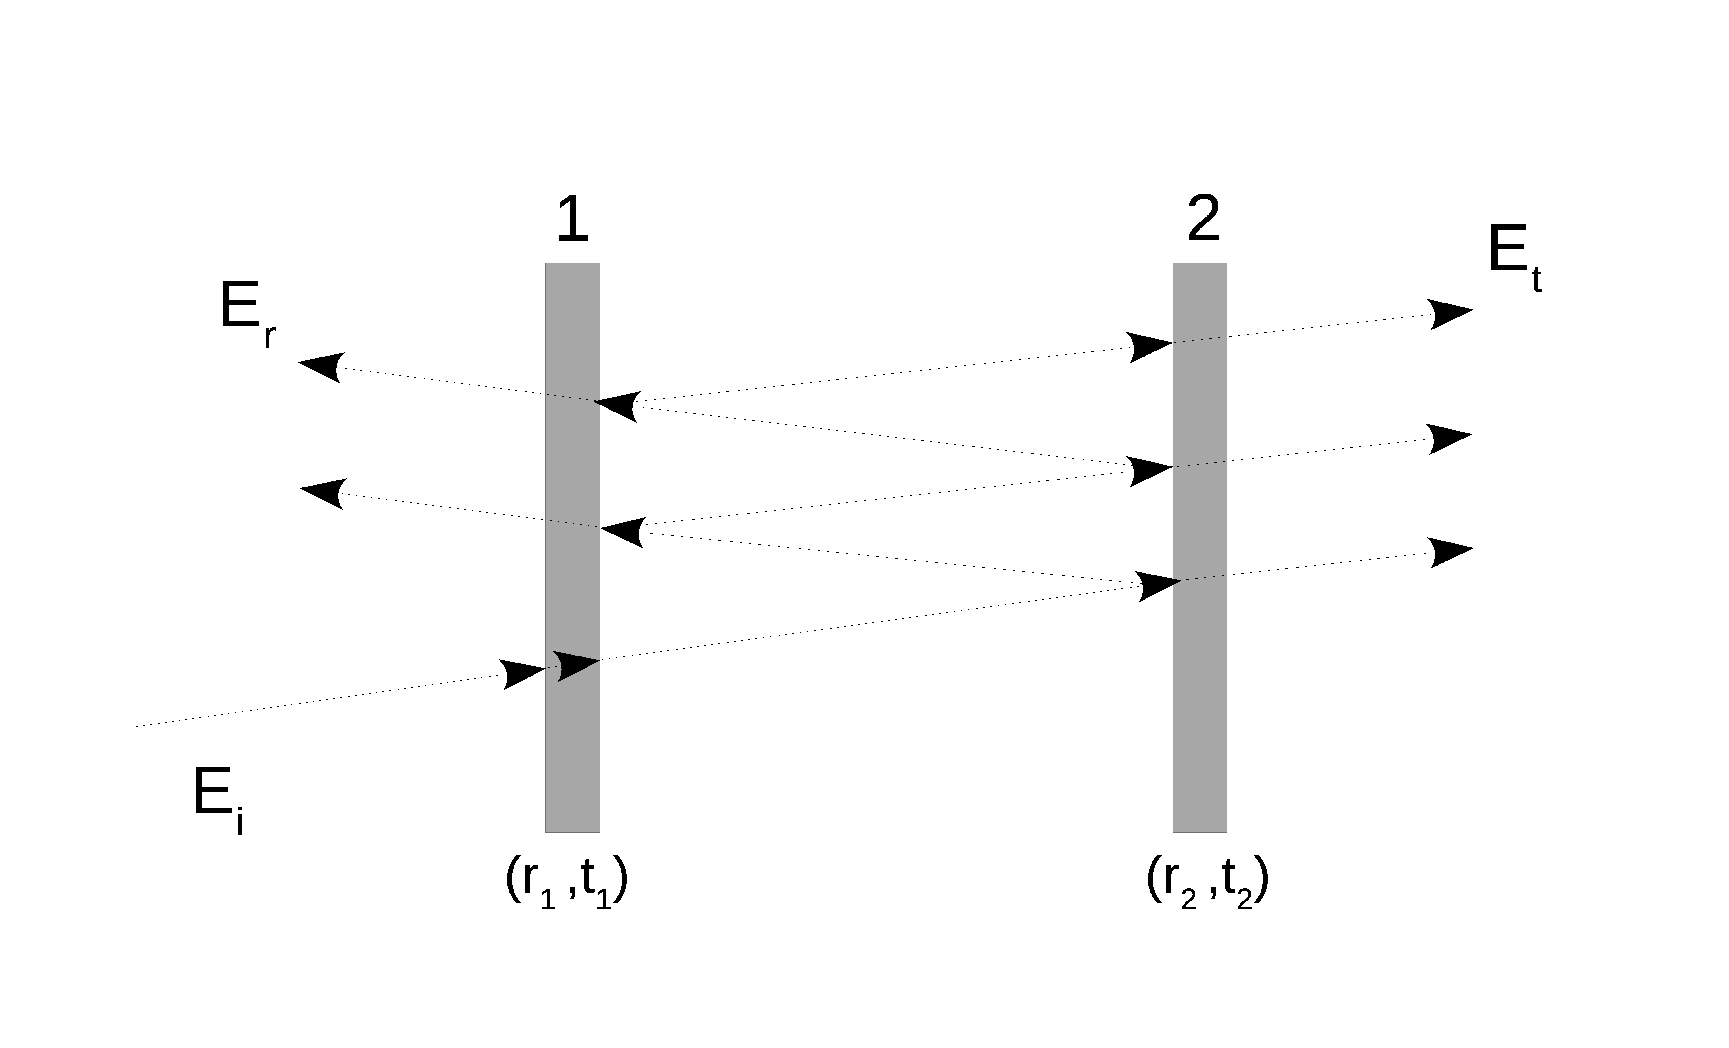
\includegraphics[width=0.65\textwidth]{Fabry_Perot_resonator.eps}
\caption{Illustrated energy diagram of a simple Fabry-Perot resonator}
\end{figure}

\newpage

\subsection{Theory of Fabry-Perot interferometer}
 If the incident energy is in the form of white coherent light then at that point the transmission and reflection coefficients depend just on the mirror reflectivities. The total reflected power comprises of the power reflected from the principal mirror in addition to all the different reflections between the mirrors that add to the reflectivity in general. In summation, the equations are: 
\begin{equation}
{\mathcal R} = R_{1} + T_{1}^2 R_{2} \sum_{m=1}^{\infty} (R_{1}R_{2})^{m-1} = \frac{R_{1} - 2R_{1}R_{2} + R_{2}}{1 - R_{1}R_{2}} _{\overrightarrow{R_{1} = R_{2} \equiv R}} \frac{2R}{1+R}
\end{equation}

Similarly, the transmitted energy in summation is:
\begin{equation}
{\mathcal T} = T_{1} T_{2} \sum_{m=1}^{\infty} (R_{1}R_{2})^{m-1} = \frac{T_{1} T_{2}}{1 - R_{1}R_{2}} _{\; \overrightarrow{R_{1} = R_{2} \equiv R}} \; \frac{T^{2}}{1-R^{2}} = \frac{1-R}{1+R}
\end{equation}

Assuming, be that as it may, the incident light comprises of a transiently lucid (monochromatic) plane wave, at that point the reflected power will be relative to the square of the reasonable total of every reflected field. Since the fields convey phase information with amplitudes added, the division of reflected and transmitted light depends not just on the mirror reflectivities, but in addition on the mirror separation and excitation wavelength. The rational 

total of fields is amplified when every one of the fields interfere constructively (in phase) and limited when they interfere destructively (out of phase). 

Phase gathers with propogation separation as $\phi(z) = \beta z$ and may likewise be gained upon communication with the mirrors. The sound forms of 

Eqs. 2.1 and 2.2 incorporate an aggregated stage factor for each round-trip that can be translated as a standardized detuning $\phi = T_{R}\omega$, where $T_{R}$ is the cavity travel time, $T_{R} = n_{eff}L/c$ for the circumference, L and effective index $n_{eff}$. Presently, $\tilde{r}$ speaks to the complex reflectivity:

\begin{multline}
\tilde{r} = r_{1} - t_{1}^{2}r_{2}\exp{(i m \phi)} \sum_{m=1}^{\infty} (r_{1}r_{2}\exp{(i m \phi)})^{m-1} \\ = \frac{r_{1} - r_{2}\exp{(i \phi)}}{1 - r_{1}r_{2}\exp{(i \phi)}} _{\; \overrightarrow{r_{1} = r_{2} \equiv r}} \; \frac{r(1-\exp{(+i \phi)})}{1-r^{2}\exp{(+i \phi)}}
\end{multline}

and $\tilde{t}$ represents the complex transmittivity:

\begin{multline}
\tilde{t} = -t_{1}t_{2}\exp{(i m \phi/2)} \sum_{m=1}^{\infty} (r_{1}r_{2}\exp{(i m \phi)})^{m-1} \\ = \frac{-t_{1}t_{2}\exp{(i m \phi/2)}}{1 - r_{1}r_{2}} _{\; \overrightarrow{r_{1} = r_{2} \equiv r}} \; \frac{-(1-r^{2})\exp{(im \phi/2)}}{1-r^{2}}
\end{multline}


The square modulus of these perplexing amounts gives the reflection ${\mathcal R}$ and transmission ${\mathcal T}$ coefficients (showin in Fig. 2.2). Antiresonant wavelengths are more emphatically reflected than in the ambiguous case, while thunderous wavelengths are transmitted $100\%$ for adjusted reflectors ($r_{1}$ = $r_{2}$). For a fixed reflect dispersing, the transmission and reflection spectra in this manner show intermittent pinnacles and valleys. Figure 3.1 presenting the transmission and reflection spectra for a lossless, adjusted Fabry– Perot resonator. The part of reflected and transmitted power for mixed up excitation is identical to the separate frightfully arrived at the midpoint of reflection and transmission over a time of the spectrum range.

\begin{figure}[h]
\centering
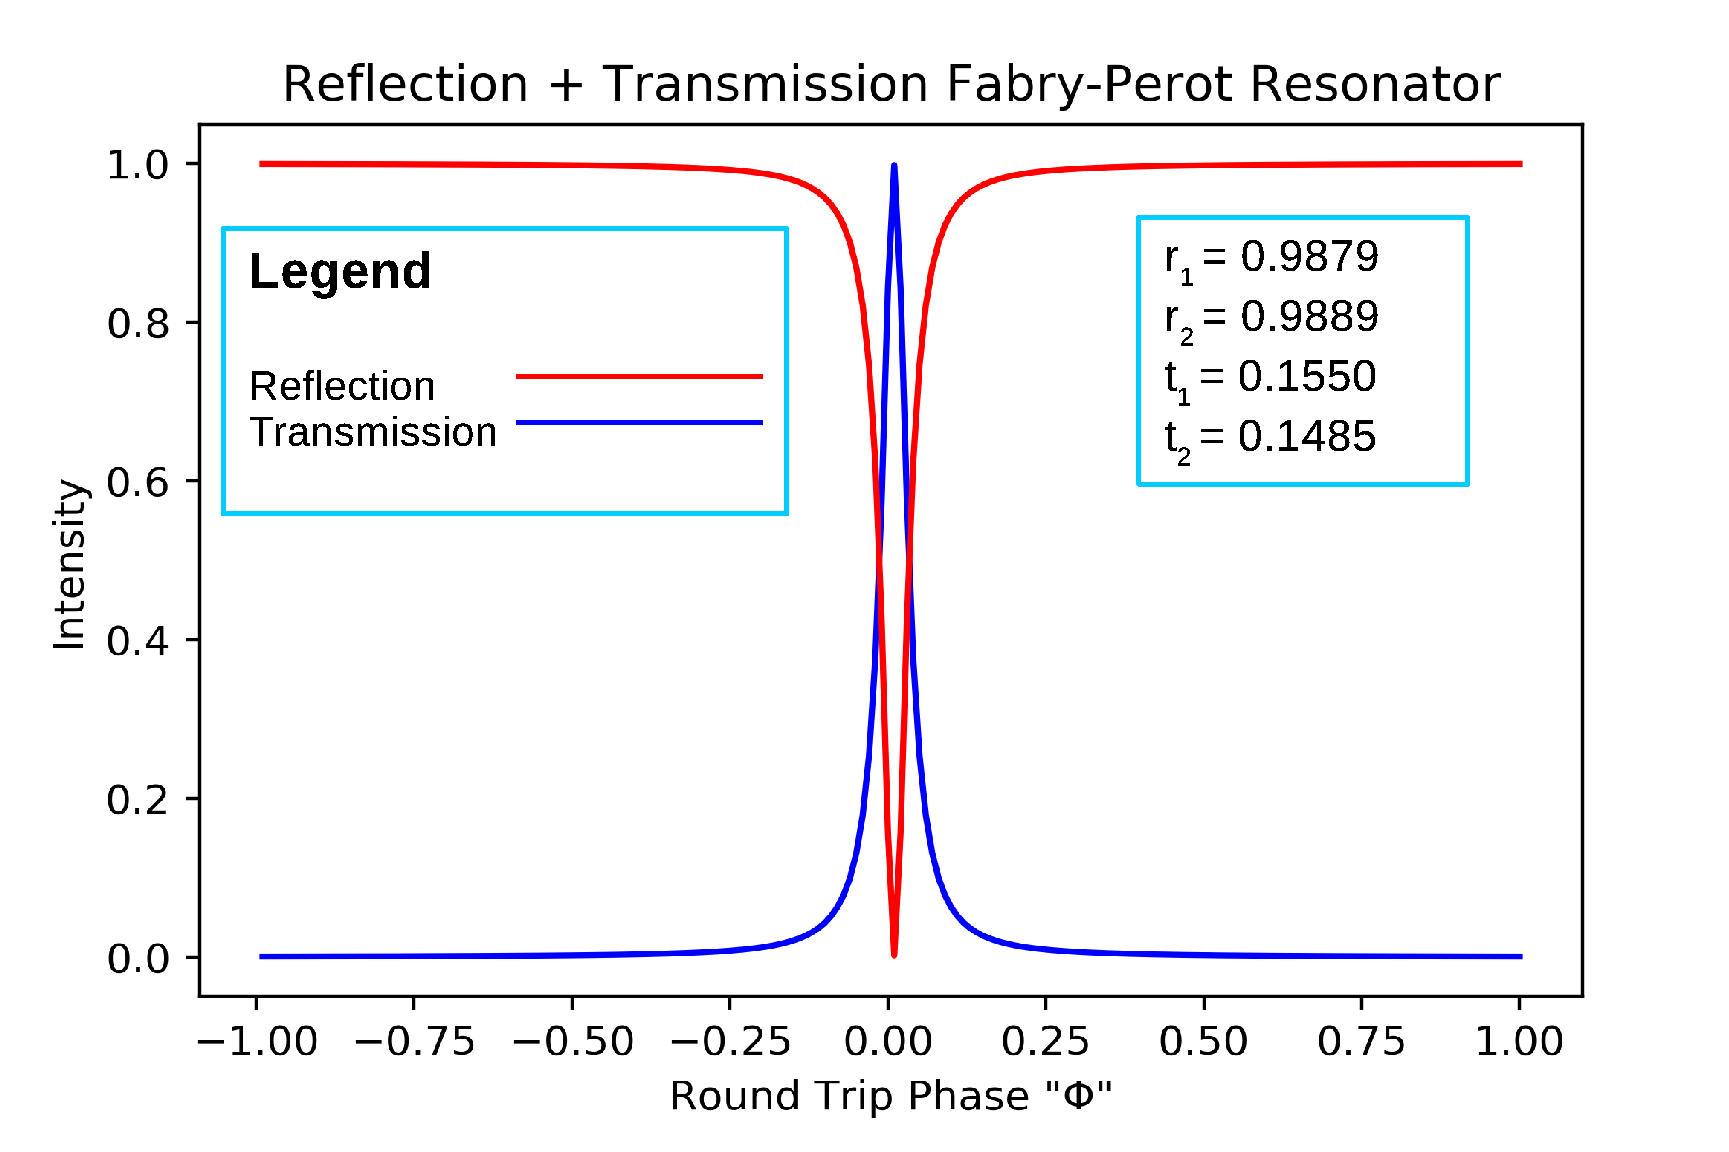
\includegraphics[width=0.5\textwidth]{R+T_FabryPerot.eps}
\caption{Transmitted and reflected field of a simple Fabry-Perot resonator}
\end{figure}

\newpage

\subsection{Finese, Q-factor}
\subparagraph{\normalfont \large The resonance condition is fulfilled when the (compelling) circumference of the ring, or for the most part the round-trip length, is equivalent to a whole number numerous of the optical wavelength inside the medium. This means a progression of Lorentzian-molded transmission bends equally dispersed in recurrence by the FSR (Free Spectral Range), with the resonance linewidth portraying the capacity time of photons inside the cavity. The photon 	lifetime can be standardized to one optical cycle, known as the quality factor (${\mathcal Q}$), or the cavity round-trip time, known as the cavity Finesse (${\mathcal F}$). The most extreme reachable Q-factor is characterized as ${\mathcal Q_{int}}$, which is the intrinsic loss of the cavity. At the point when the resonator is coupled to the outer world, the Q-factor further decreases because of the loss imported by the coupler (${\mathcal Q_{ext}}$). Thus the last quality factor ${\mathcal Q_{load}}$ is comprised of these two parts: ${\mathcal Q_{load}^{-1}}$ = ${\mathcal Q_{int}^{-1}}$ + ${\mathcal Q_{ext}^{-1}}$.}


\section{Ring Geometry Resonators}
In this section, I will discuss different kinds of ring shaped resonators whose principle is pretty much similar to the Fabry-Perot resonator and are more simple to make. Basically, a ring resonator is a simple waveguide which is turned in the shape of a ring. This allows it to exhibit resonant behavior on very specific frequencies. The light is coupled inside the ring due to the phenomenon of total internal reflection and interference. This kind of behaviour is noticed in all kind of classical waves, such as sound waves, which was observed inside a large cathedral's halls, thus it was named whispering galleries. Also, these resonators can be made using different material but in this thesis, we used semi-conductor silicon as the primary material. 

\subsection{All-Pass Ringresonator}
A straightforward ring resonator is made by taking one yield of a conventional directional coupler and bolstering it once again into one input. Such a device displays periodic cavity resonance (reverberation) when light navigating the ring procures a phase move relating to a number numerous of 2$\pi$ radians. The resonator is numerically defined from two parts: a coupling quality and an input way. In opposition to the limitless entirety inferences performed before for the Fabry– Perot and Gires– Tournois, in which we expected steadystate task and coordinating fields and derived basic spectral properties. Although, both strategies are similarly substantial, the field-coordinating technique has the benefit of simplicity.
\begin{figure}[h]
\centering
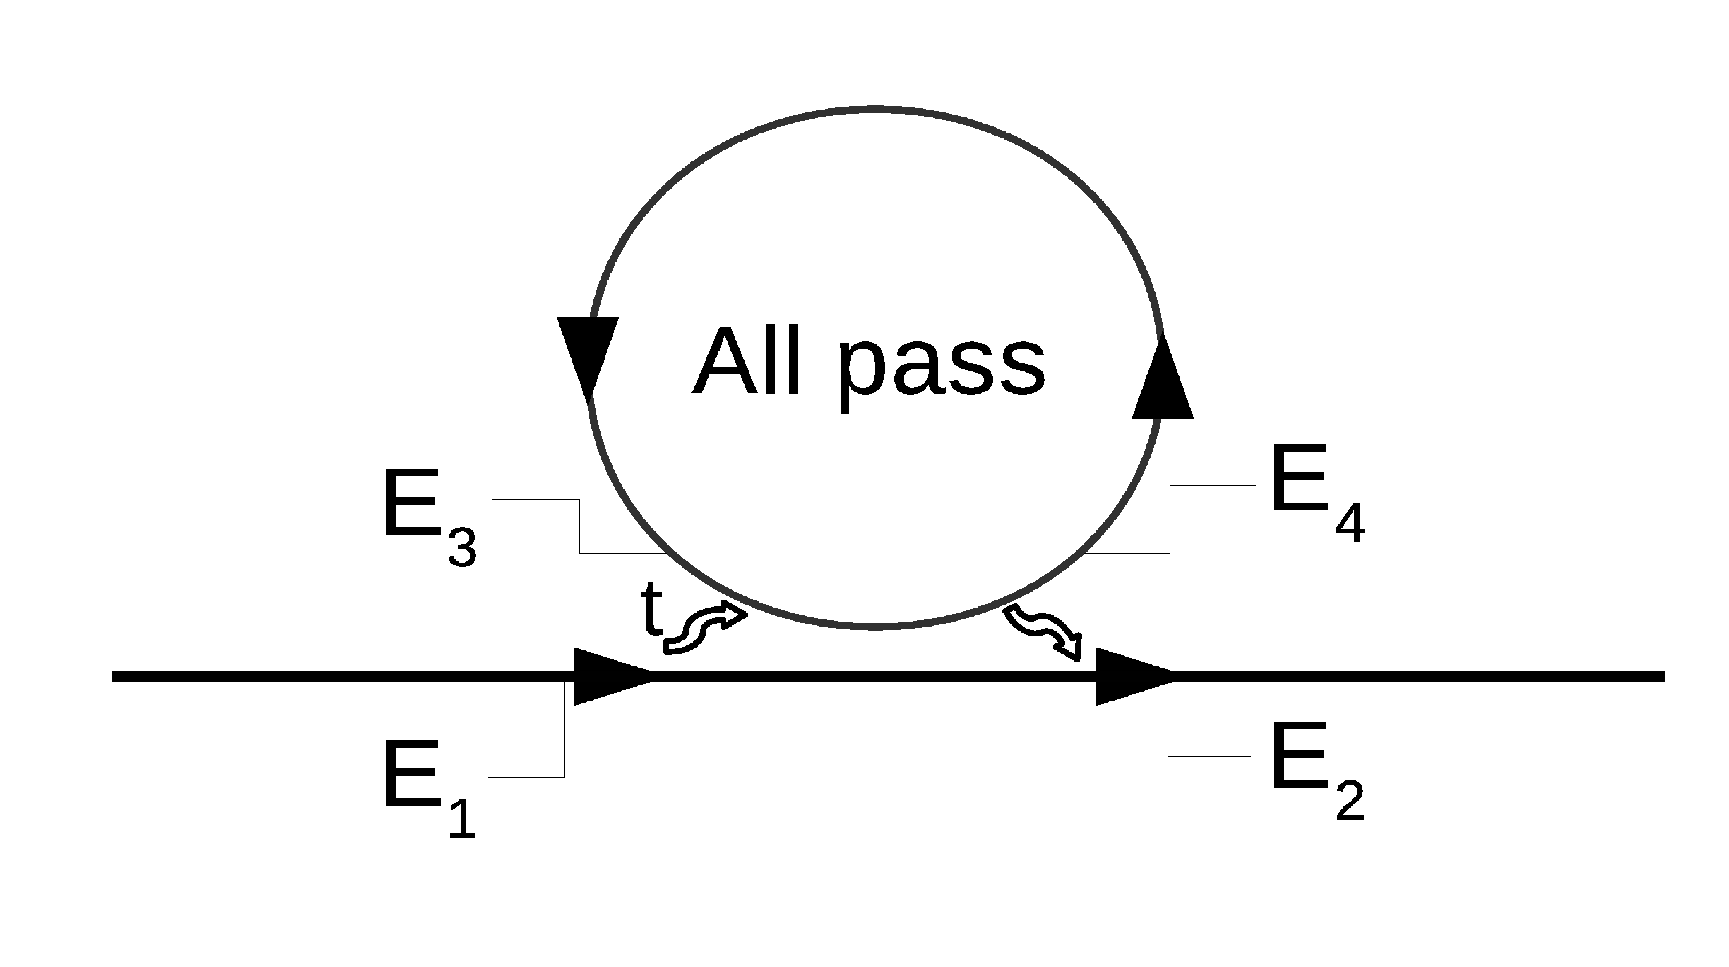
\includegraphics[width=0.5\textwidth]{all_pass_resonator.eps}
\caption{Illustrated fields of an all pass resonator}
\end{figure}
\subsection{Add-Drop Ringresonator}
The immediate waveguide similarity of a free-space Fabry– Perot is gotten by including a second guide that side-couples to the resonator as in Fig. 1.4.
Since this setup acts as a tight band abundancy channel that can include or drop a recurrence band from an approaching sign, it is regularly named an add– drop filter.
\begin{figure}[h]
\centering
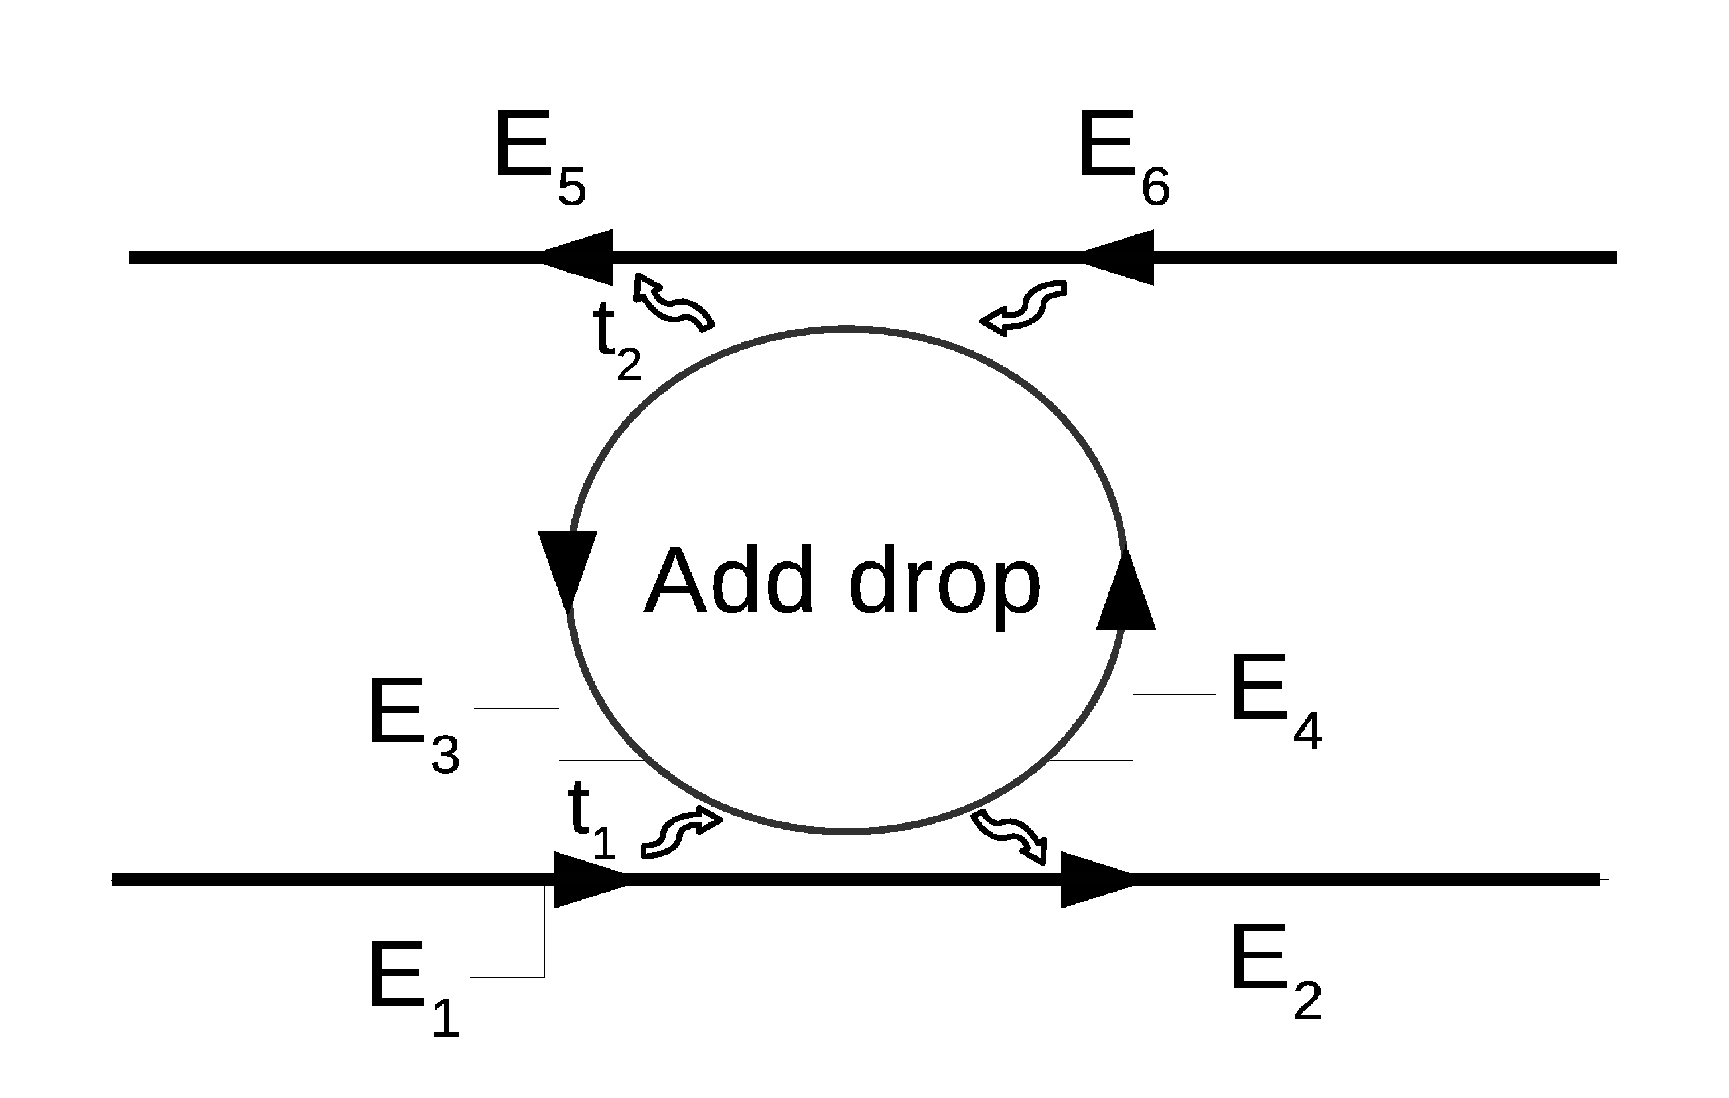
\includegraphics[width=0.5\textwidth]{add_drop_resonator.eps}
\caption{Illustrated fields of an add drop resonator}
\end{figure}
\subsection{Coupled Ringresonator}
A simple case as an assymeteric Fabry-Perot resonator, a coupled ring resonator has another ring above the first ring of the all pass resonator. This arrangement shows coupling between the two resonators (rings) and show different behaviour. 
\begin{figure}[h]
\centering
\includegraphics[width=0.45\textwidth]{couple_ring_resonator.eps}
\caption{Illustrated fields and geometry of a coupled ring resonator}
\end{figure}
\newpage

\section{Gain incorporation in Resonators}
Light, when travels through a medium, loses its intensity exponentially. This law is called the $Beer's law$ for electromagnetic intensity. But some mediums, whose refractive index is such as they oppose the exponential decay of the light and rather increase the intensity in the propogation through the medium, are called gain medium. We can use these gain mediums and build a microresonators from them to observe different quantum optical phenomenons. First I will explain a bit how gain work.


\subsection{Beer's Law}
 binary floating-point arithmetic and some concepts from numerical analysis.Most of the time, using mpmath is simply a matter of setting the desired precision and entering a formula. For verification purposes, a quite (but not always!) reliable technique is to calculate the same thing a second time at a higher precision and verifying that the results agree.
\subsection{Beer's law study as gain}
To perform more advanced calculations, it is important to have some understanding of how mpmath works internally and what the possible sources of error are. This section gives an overview of arbitrary-precision binary floating-point arithmetic and some concepts from numerical analysis.Most of the time, using mpmath is simply a matter of setting the desired precision and entering a formula. For verification purposes, a quite (but not always!) reliable technique is to calculate the same thing a second time at a higher precision and verifying that the results agree.
\section{Gain medium}
To perform more advanced calculations, it is important to have some understanding of how mpmath works internally and what the possible sources of error are. This section gives an overview of arbitrary-precision binary floating-point arithmetic and some concepts from numerical analysis.
 
\chapter{Gain Controlled Coupled-resonator-induced Transparecy and Absorption}
\section{Electromagnetically Induced Transparency}
Electromagnetically Induced Tranparency is a well known phenomenon in atomic physics but its all-optical analogue has generated a lot of interest in this beautiful natural phenomenon. Basically, EIT is a transparency window in transmission and absorption spectrum. This transparency window is the result of fano interference amoung different transition pathways. There is another similar concept which is known as Autler-Townes Splitting ATS, which also shows a transparency window but it is the result of strong field-driven interactions which causes the energy levels to split.

EIT also enables us to hold control over the optical response of the medium. Basically, EIT is the result of having a strong connection between the light and the matter. Amplitudes of different pathways interfere due to quantum interference effects. These can be used in applications such as all-optical switching, slow light, optical sensing, light storage and quantum information processing.

In photonics, EIT is said to be observed in plasmonic structures, photonic crystals, whispering gallery mode micro cavities and coupled ring micro resonators. These devices can be summed up under one name, photonic devices and by seeing such effects we can say that we can get control of how information and energy travel through our device.

\subsection{EIT in Atoms}
For EIT to happen classically, one may assume that all the oscillating atoms in the medium have came to a hault just to neutralize the incoming field effect and thus these electrons does not contribute in the dielectric of the material. But atoms are small and must be treated quantum mechanically, in which we deal with probability amplitudes and expected value of electron's position. 
\subsection{Three level Atoms}
In a three level system, what really happens quantum mechanically, without disrupting the escence of classical phenomenons, The probability amplitudes of level $\ket{3}$ is driven by two terms in the system. One is being the probability amplitude of the ground state $\ket{1}$ and the other is the oppositely phased and is the probability amplitude of the state $\ket{2}$. These both driving forces are opposite in signs but equal in magnitudes and have a frequecy $\omega_{p}$ and are so balanced that probabilty amplitude of state $\ket{3}$ and the expected value of the amplitude of the sinosoidal motion at every frequency that has been applied is zero. 
One may ask how that opposite phase for transition from the coherent states $\ket{1} \to \ket{2}$ along with the applied field $\omega_{c}$, makes absolute cancellation? Because, we use the laser pulses that generates fast enough laser photons that the phase of transitions is maintain and is the correct phase for cancellation. 

\begin{figure}[h]
\centering
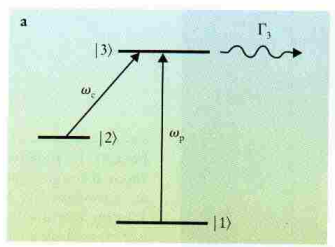
\includegraphics[scale=0.5]{EIT_3levl_atom.png}
\caption{A three-level system where level 3 decays with $\Gamma_{3}$ to states outside the system. [1]}
\end{figure}


\section{Coupled Resonator Induced Transparency (CRIT)}
We can observe EIT in coupled resonator systems as well as in other optical systems like whispering gallery resonators but the scope of this thesis is limited to ring resonators systems only. This kind of geometry (That we discussed in section 2.4) has been promising since a long time in the field of photonics. EIT can be observed in this system by mostly the explaination of classical wave travel and quantum fluctuations. The traveling photon is coupled inside the first ring through evanescent wave and travels inside the ring and acquires a phase shift equal to the round trip inside the optical cavity. When the light source and the phase shifted intracavity field matches so as that the constructive interference is amplified i-e their phases matches perfectly, then at those frequency there is a transparency window in the absorption spectrum i-e a narrow dip, or we see a sharp peak in the transmission spectrum. [2] 

\subsubsection{Transmittance}
Figure 3.2 displays the plot of transmitted intensity vs frequency detuning in a coupled resonator system as shown in fig. 2.16. The parameters used here are couplings $r_{1} = 0.9$ and $r_{2} = 0.999$ and attenuations $a_{1} = 0.88$ and $a_{2} = 0.9999$ for ring 1 and 2 respectively. [2]

\begin{figure}[h]
\centering
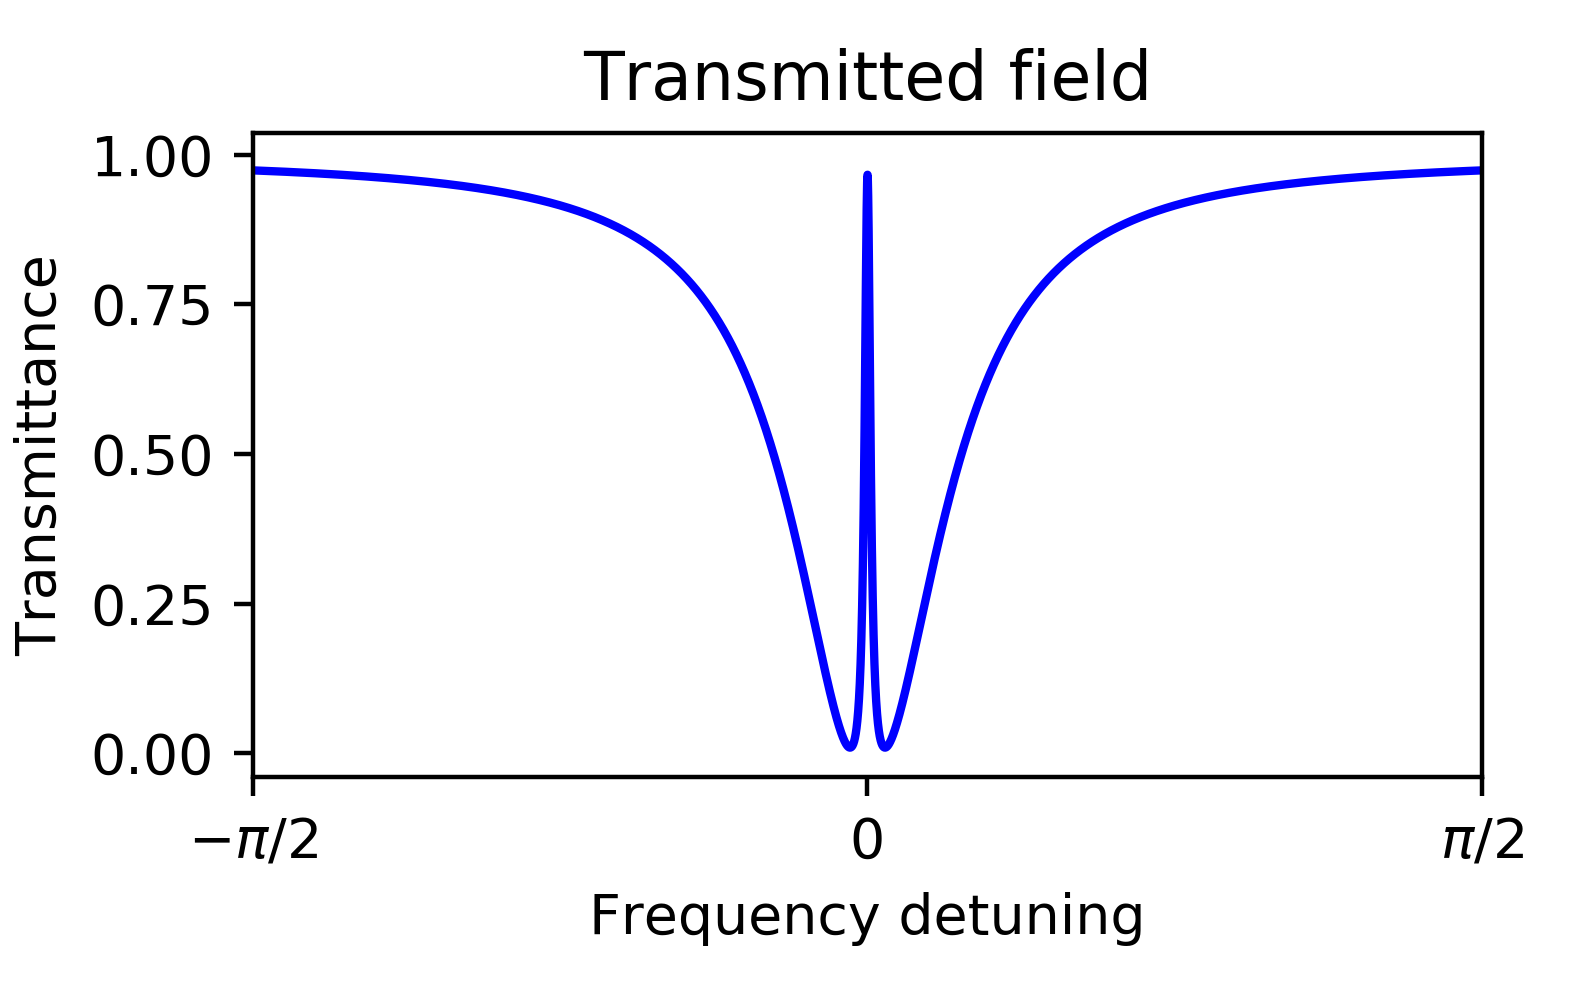
\includegraphics[scale=1]{coupled_ring_EIT1.png}
\caption{EIT observed in a 2 ring resonator system.}
\end{figure}

\subsubsection{Phase}

Now let us look at the phase response of such coupled resonator system. Figure 3.3 shows effective phase of the system in red and Figure 3.4 shows the coupling phase which is the phase between the two coupled rings, in yellow. 

\begin{figure}[h]
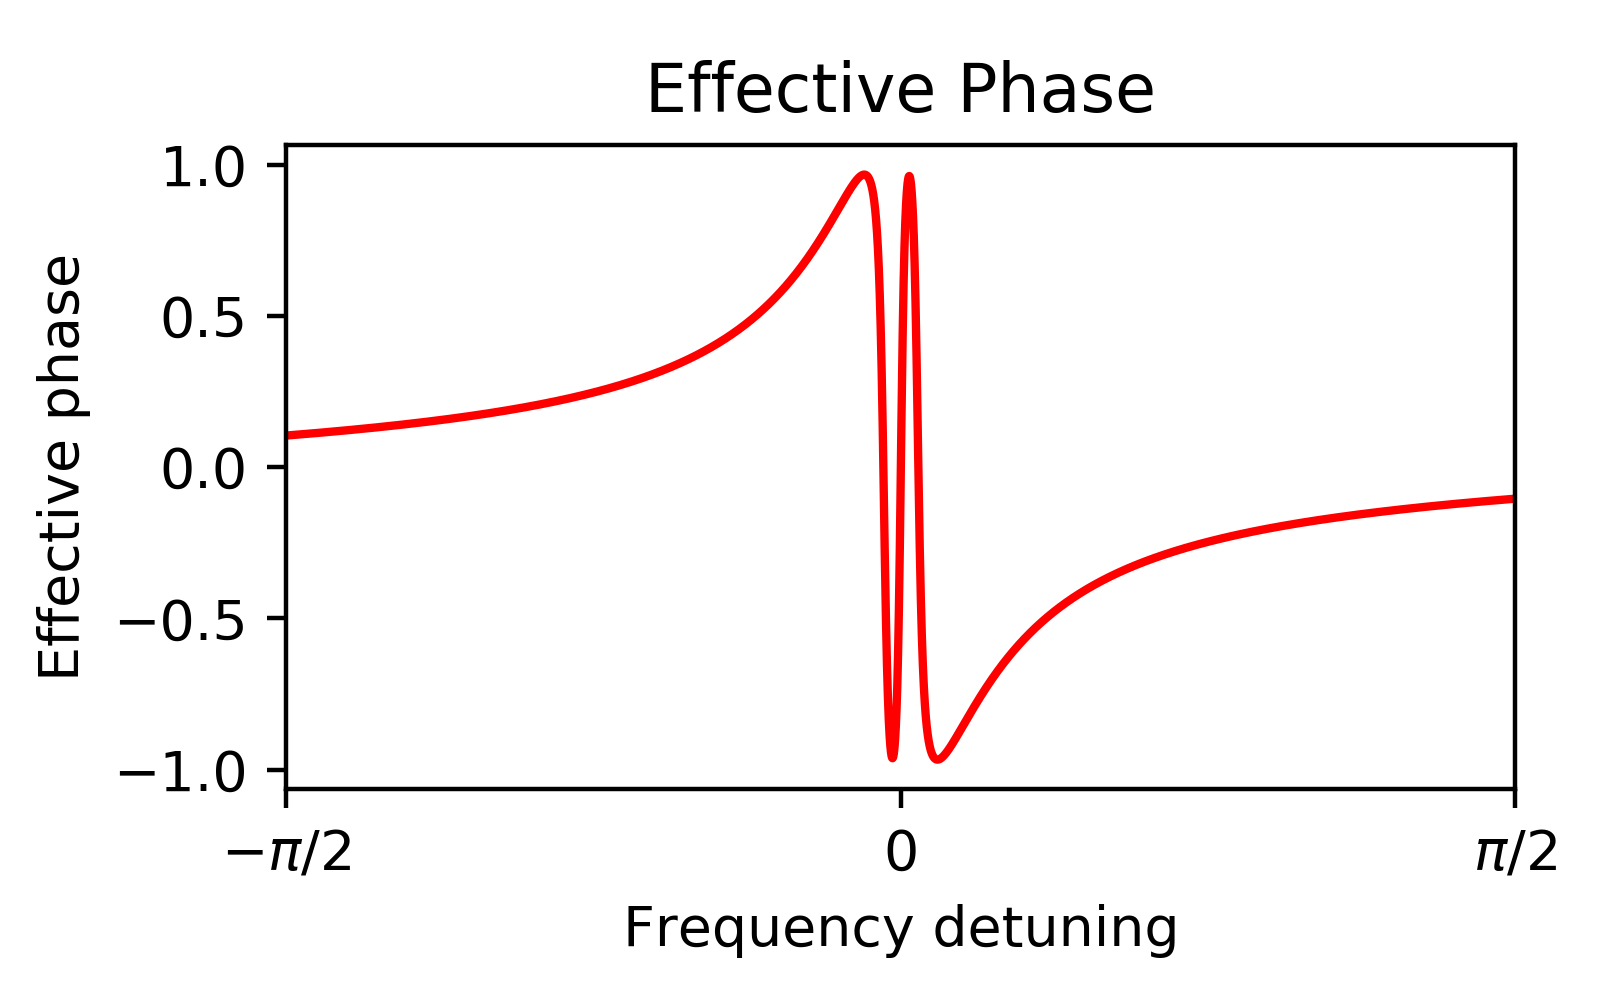
\includegraphics[scale=0.75]{coupled_ring_EIT1_phase.png}
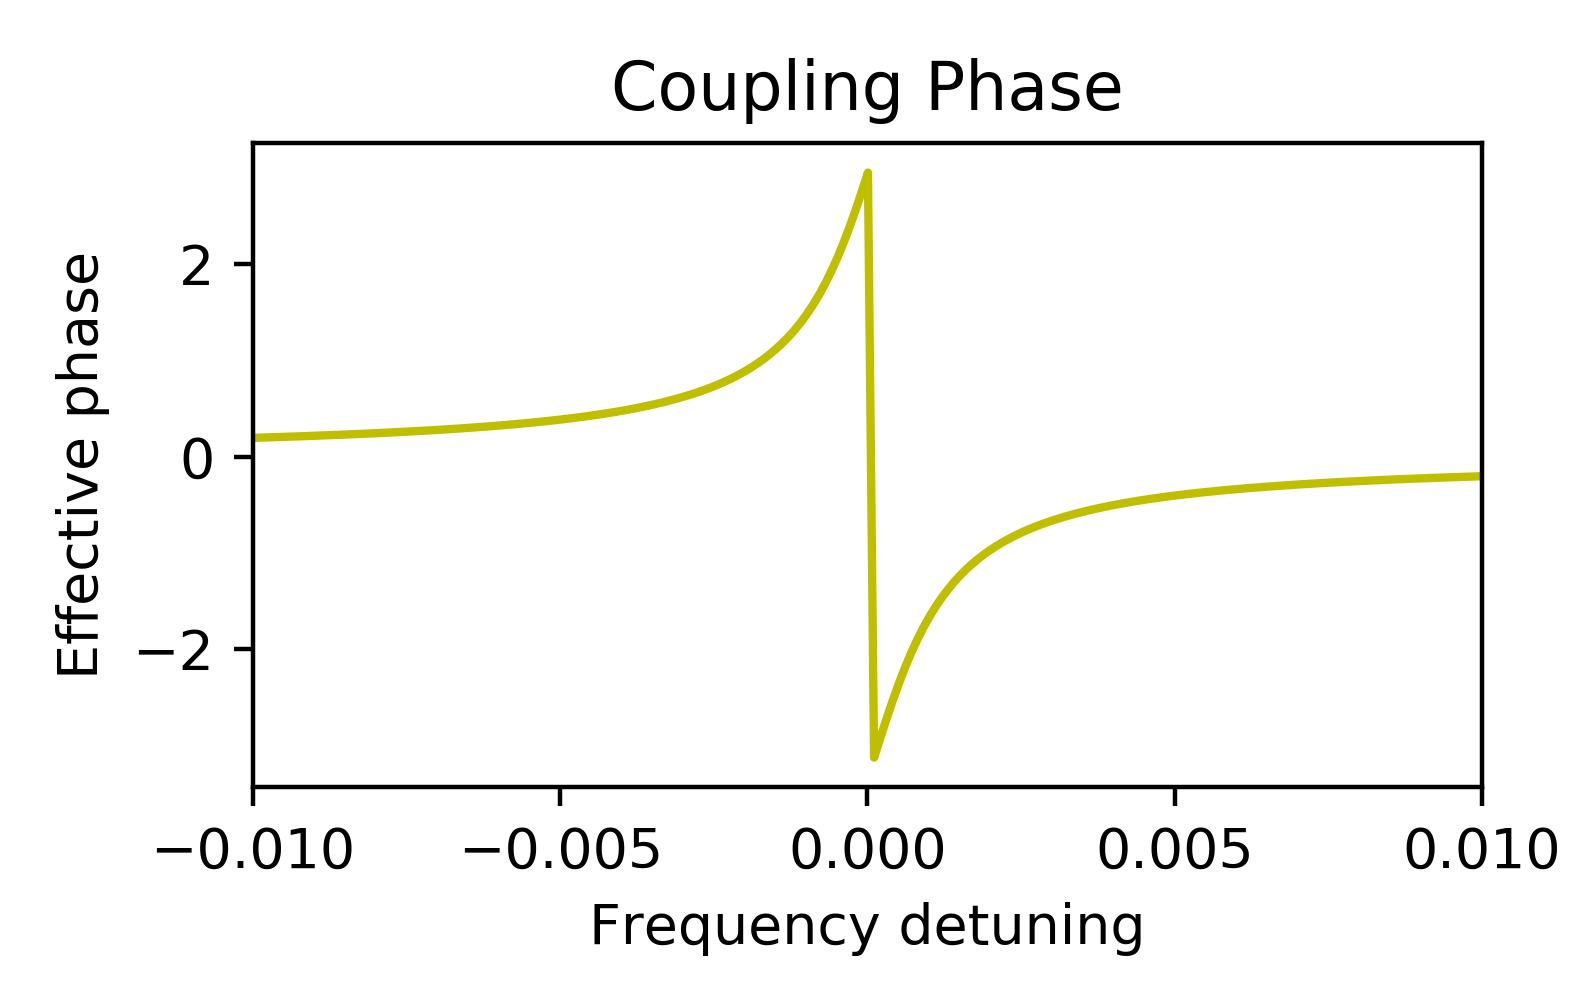
\includegraphics[scale=0.75]{coupled_ring_EIT1_coupling.png}
\caption{Effective phase of the system in red and coupling phase shown in yellow vs frequency detuning.}
\end{figure}

\subsubsection{Effective Phase derivative}
Figure 3.4 shows the derivative of the phase of the system which gives us great information about the group index and group velocity of the system. 
\begin{figure}[h]
\centering
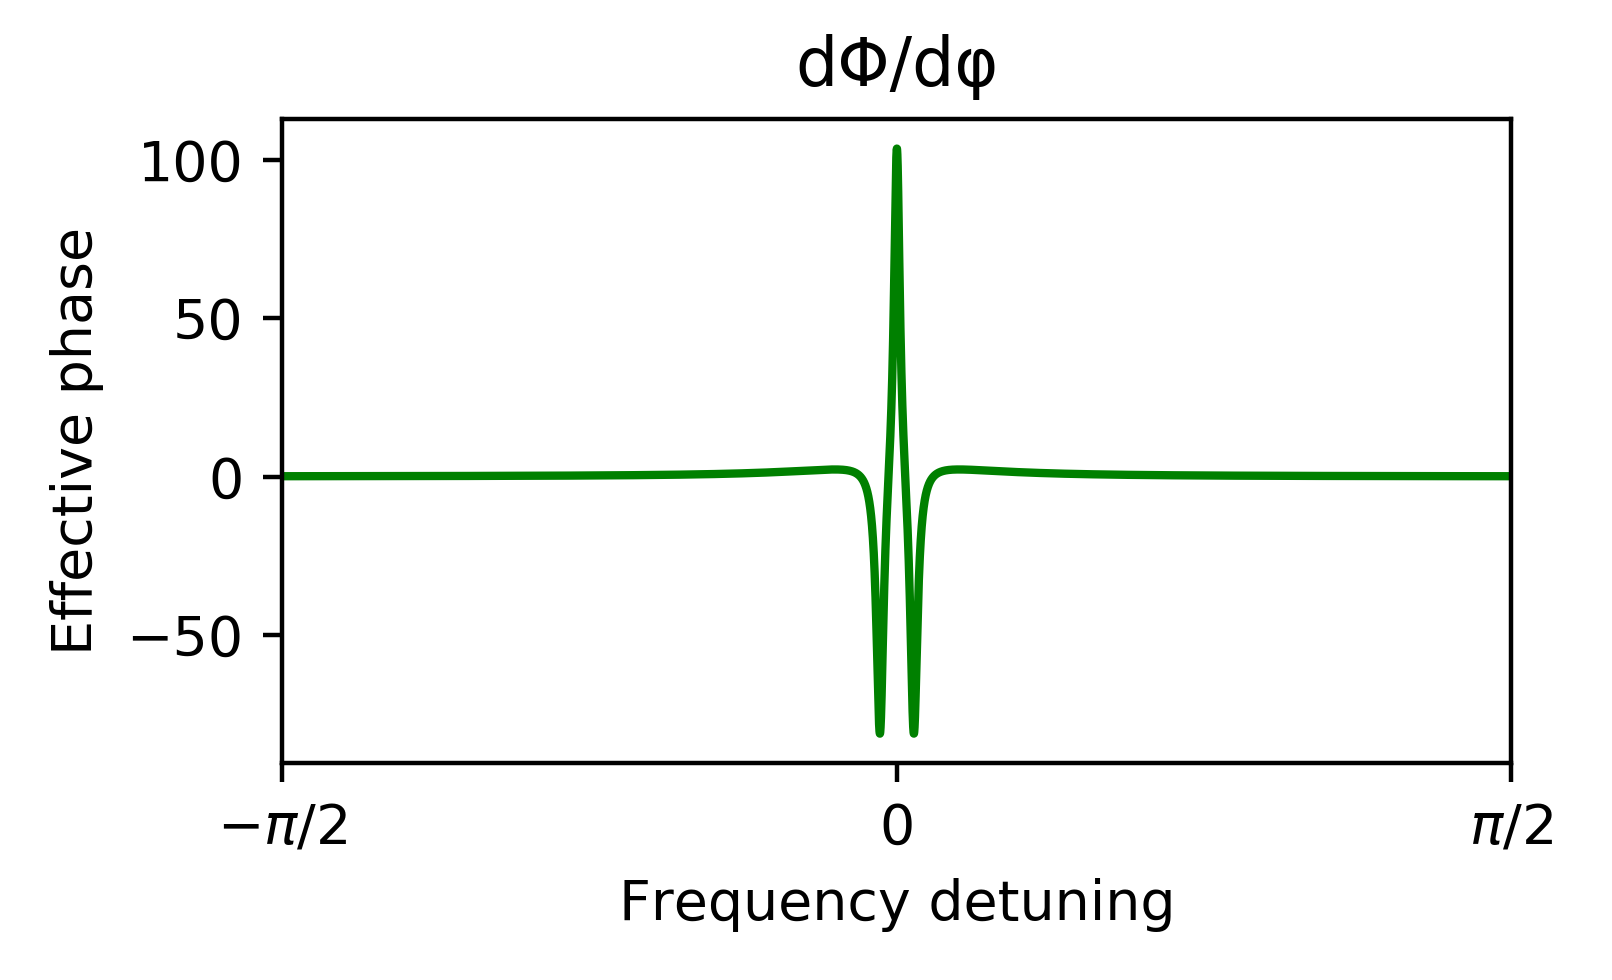
\includegraphics[scale=1]{coupled_ring_EIT1_deri.png}
\caption{Derivative of the phase of the system vs frequency detuning.}
\end{figure}


\subsection{CRIT with gain}
As before, now we are going to observe what changes does the system has when we introduce gain in it. This can be introduced by pumping some monochromatic light source or a laser, in either one of the rings which will drastically incompensate the losses inside the resonator and will increase the overall output transmission of the system even above the incident light source. 
\subsubsection*{Results}
To perform more advanced calculations, it is important to have some understanding of how mpmath works internally and what the possible sources of error are. This section gives an overview of arbitrary-precision binary floating-point arithmetic and some concepts from numerical analysis.Most of the time, using mpmath is simply a matter of setting the desired precision and entering a formula. For verification purposes, a quite (but not always!) reliable technique is to calculate the same thing a second time at a higher precision and verifying that the results agree.

To perform more advanced calculations, it is important to have some understanding of how mpmath works internally and what the possible sources of error are. This section gives an overview of arbitrary-precision binary floating-point arithmetic and some concepts from numerical analysis.


\section{EIA concepts}
To perform more advanced calculations, it is important to have some understanding of how mpmath works internally and what the possible sources of error are. This section gives an overview of arbitrary-precision binary floating-point arithmetic and some concepts from numerical analysis.To perform more advanced calculations, it is important to have some
\subsection{EIA in atoms}
 understanding of how mpmath works internally and what the possible sources of error are. This section gives an overview of arbitrary-precision binary floating-point arithmetic and some concepts from numerical analysis.To perform more advanced calculations, it is important to have some understanding of how mpmath works internally and what the possible sources of error are. 
\subsection{EIA Quantum phenomena} 
 This section gives an overview of arbitrary-precision binary floating-point arithmetic and some concepts from numerical analysis.To perform more advanced calculations, it is important to have some understanding of how mpmath works internally and what the possible sources of error are. This section gives an overview of arbitrary-precision binary floating-point arithmetic and some concepts from numerical analysis.To perform more advanced calculations, it is important to have some understanding of how mpmath works internally and what the possible sources of error are. This section gives an overview of arbitrary-precision binary floating-point arithmetic and some concepts from numerical analysis.To perform more advanced calculations, it is important to have some understanding of how mpmath works internally and what the possible sources of error are.
\section{EIA in resonators} 
 
  This section gives an overview of arbitrary-precision binary floating-point arithmetic and some concepts from numerical analysis.To perform more advanced calculations, it is important to have some understanding of how mpmath works internally and what the possible sources of error are. This section gives an overview of arbitrary-precision binary floating-point arithmetic and some concepts from numerical analysis.
  
\subsection{Coupled resontors induced Absorption}

To perform more advanced calculations, it is important to have some understanding of how mpmath works internally and what the possible sources of error are. This section gives an overview of arbitrary-precision binary floating-point arithmetic and some concepts from numerical analysis.To perform more advanced calculations, it is important to have some understanding of how mpmath works internally and what the possible sources of error are. This section gives an overview of arbitrary-precision binary floating-point arithmetic and some concepts from numerical analysis.
\section{CRIA with gain}
To perform more advanced calculations, it is important to have some understanding of how mpmath works internally and what the possible sources of error are. This section gives an overview of arbitrary-precision binary floating-point arithmetic and some concepts from numerical analysis.To perform more advanced calculations, it is important to have some understanding of how mpmath works internally and what the possible sources of error are. This section gives an overview of arbitrary-precision binary floating-point arithmetic and some concepts from numerical analysis.


\newpage
\section*{References}
\addcontentsline{toc}{section}{References}

\paragraph{\normalfont \large $[1]$ Electromagnetically Induced Transparency, Stephen E. Harris, Physics Today, July 1997 \\ 
\\$[2]$ Coupled-resonator-induced transparency, PHYSICAL REVIEW A 69, 063804 (2004)
\\$[3]$ What is and what is not electromagnetically induced transparency in whispering-gallery microcavities, DOI:10.1038/ncomms6082, Published 24 Oct 2014 \\
\\$[4]$  Induced transparency and absorption in coupled whispering gallery microresonators, PHYSICAL REVIEW A 71, 043804, published 5 April 2005\\
\\$[5]$  }
 
\chapter{Cascaded Resonances in Three Coupled Resonators}
In this chapter, we will now extend our study on composite resonator systems. Such as, we will increase the number of resonators in our system. These structures, that will be discussed here, were not optimized to achieve enhanced dispersion. Rather the purpose of these analyses is to demonstrate the versatility and distinct optical characteristics of cascaded resonances which are obtained by cascading three resonators (Fig. 4.1). For the scope of this thesis, the system will consist of ring-shaped resonators and thus we will study properties of such ring resonators and their mutual coupling effects.
\section{Triple Ring Resonator System}
Now we introduce a new resonator geometry. Basically, we are to simply add another ring above the coupled two resonator system which was discussed in greater detail Chapter 3. Now we have a three-resonator system with each having their own distinct resonant frequencies. These resonators show distinct properties due to the introduction of an additional ring with a higher Quality-factor, coupled to the two resonator system. This allows us to observe multiple resonances and observe phenomenons like CRIT and CRIA with another perspective. This also enables us to simultaneously measure these effects in a single system and thus obtain versatile transmission and dispersion.

The illustration in Fig. 4.1 shows us that the three rings are mutually coupled to each other and only the first ring is coupled to the optical waveguide. The incident energy from the input is labeled as $E_{1}$ which couples to the first resonator due to evanescent coupling. The energy is then transferred to $E_{3}$. This energy travels the first ring and is again coupled into the  as $E_{5}$ and then again into the third resonator with energy $E_{7}$. Then it loops back into the waveguide as $E_{8}$, $E_{6}$ and $E_{4}$ respectively to couple back to the waveguide, each acquiring a distinct phase shift and outputs the signal with energy $E_{2}$. Here, $E_{3}$ and $E_{4}$ describes the circulating fields of the first resonator. Evanescent coupling between the first and the second resonator results in the circulating fields of the resonator two labeled $E_{5}$ and $E_{6}$. A similar mechanism leads to the excitation of the resonant mode of the third cavity, with circulating fields described by $E_{7}$ and $E_{8}$.

\begin{figure}[h]
\centering
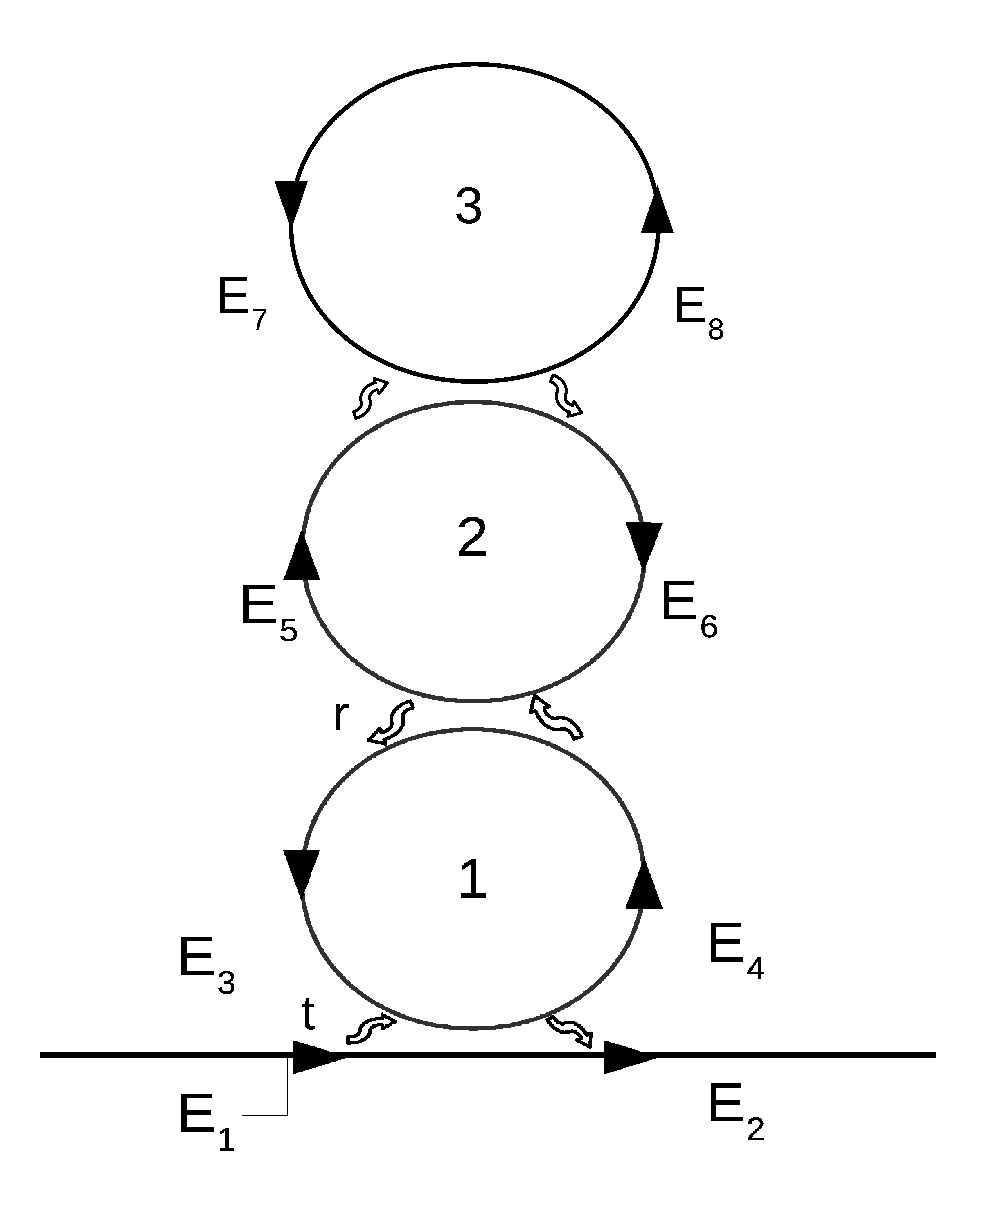
\includegraphics[scale=0.45]{triple_ring_resonator.eps}
\caption{Basic illustration of three ring resonator geometery along with its respective fields. Here, first resonator is labeled as 1, second is labeled as 2, and third is labeled as 3.}
\end{figure}

\subsection{Transmission and Phase relations}
The complex transmitivity and its respective phase can be determined by equations 4.1 and 4.2 respectively. 

\begin{equation}
\frac{E_{t}}{E_{i}} = \frac{r_{1} - a_{1} \, r_{12} \, e^{i\phi_{1}}}{1 - r_{1}\, r_{12}\, a_{1}\, e^{i\phi_{1}}}
\end{equation}

where, 
\begin{align*}
r_{12} = \frac{r_{2} - a_{2}\, r_{23}\, e^{i \phi_{2}}} {1 - r_{2} r_{23}\, a_{2}\, e^{i \phi_{2}}} 
\end{align*}
and,
\begin{align*}
r_{23} = \frac{r_{3} - a_{3}\, e^{i \phi_{3}}} {1 - r_{3}\, a_{3}\, e^{i \phi_{3}}} 
\end{align*}

Similarly, the effective phase of the complex transmitivity is given by:

\begin{equation}
\phi_{eff} = \arctan[{\frac{r_{1} |r_{12}| a_{1} \sin{(\phi_{1} + \phi_{12})}}{1 - |r_{12}| a_{1} \cos{(\phi_{1} + \phi_{12})}}}] - \arctan[{\frac{|r_{12}| a_{1} \sin{(\phi_{1} + \phi_{12})}}{r_{1} - |r_{12}| a_{1} \cos{(\phi_{1} + \phi_{12})}}}]
\end{equation}

Now we use these equations to observe characteristics of triple cavity resonances.

\section{Passive Three Resonator Results}
We can obtain very interesting results from a passive three resonator systems some of which are discussed in this section. Fig. 4.2 displays CRIT inside a CRIA resonance hence negative group index and fast light are obtained on resonant frequencies while large values of subluminal group indexes are clearly apparent at the off-resonance transmission. When resonator two is allowed to couple with the third resonator, due to its effects there is an on-resonance peak inside the CRIA dip. These cascaded resonances can help play an important role in the tunability of fast and slow light and/or in large and small absorption of resonant frequencies. This may lead to new applications in communication technology and related fields. These kinds of effects which were observed in atomic systems had shortcomings due to a large amount of absorption and had low-temperature maintenance problems. Now, these effects can be observed in photonic resonators which are operatable at room temperatures.
\subsection{CRIT inside CRIA}
In Fig. 4.2, we see that the transmission spectrum looks like a CRIA dip, meaning it will display the properties of CRIA. The system parameters are given as, $r_{1} = 0.898945$, $r_{2} = 0.999958$, and $r_{3} = 0.999999$. The $\mathcal{Q}-factors$ are $1\times10^{5}, 1\times10^{6}$ and $1\times10^{7}$ for first second and third resonator respectively. When we zoom into the graph (as shown on the right), we observe that there is another peak rising within the CRIA, showing the feature due to the third resonance of the third resonator. Thus now we have CRIT inside a CRIA transmission. This will allow us to have transmission intensity larger while maintaining the characteristics of CRIA dispersion. Now we can have more light in CRIA mediate transmission. This means we can have fast light dispersion on on-resonant frequencies, which can be enhanced by adjusting mutual coupling of the resonators.

The effective phase of the system is shown in red where we see a normal curve stretching from positive to negative horizontal and vertical axes. But when we zoom into the middle of the curve, we see two features instead of one which characterize the presence of three cavities. The zoomed version is shown on the right in Fig. 4.2 and it displays a negative slope on resonance meaning the light we are receiving in the transmission is fast light. Thus we conclude that we have superluminal light along with large transmission owing to cascaded CRIT and CRIA.

\begin{figure}[t]
\centering
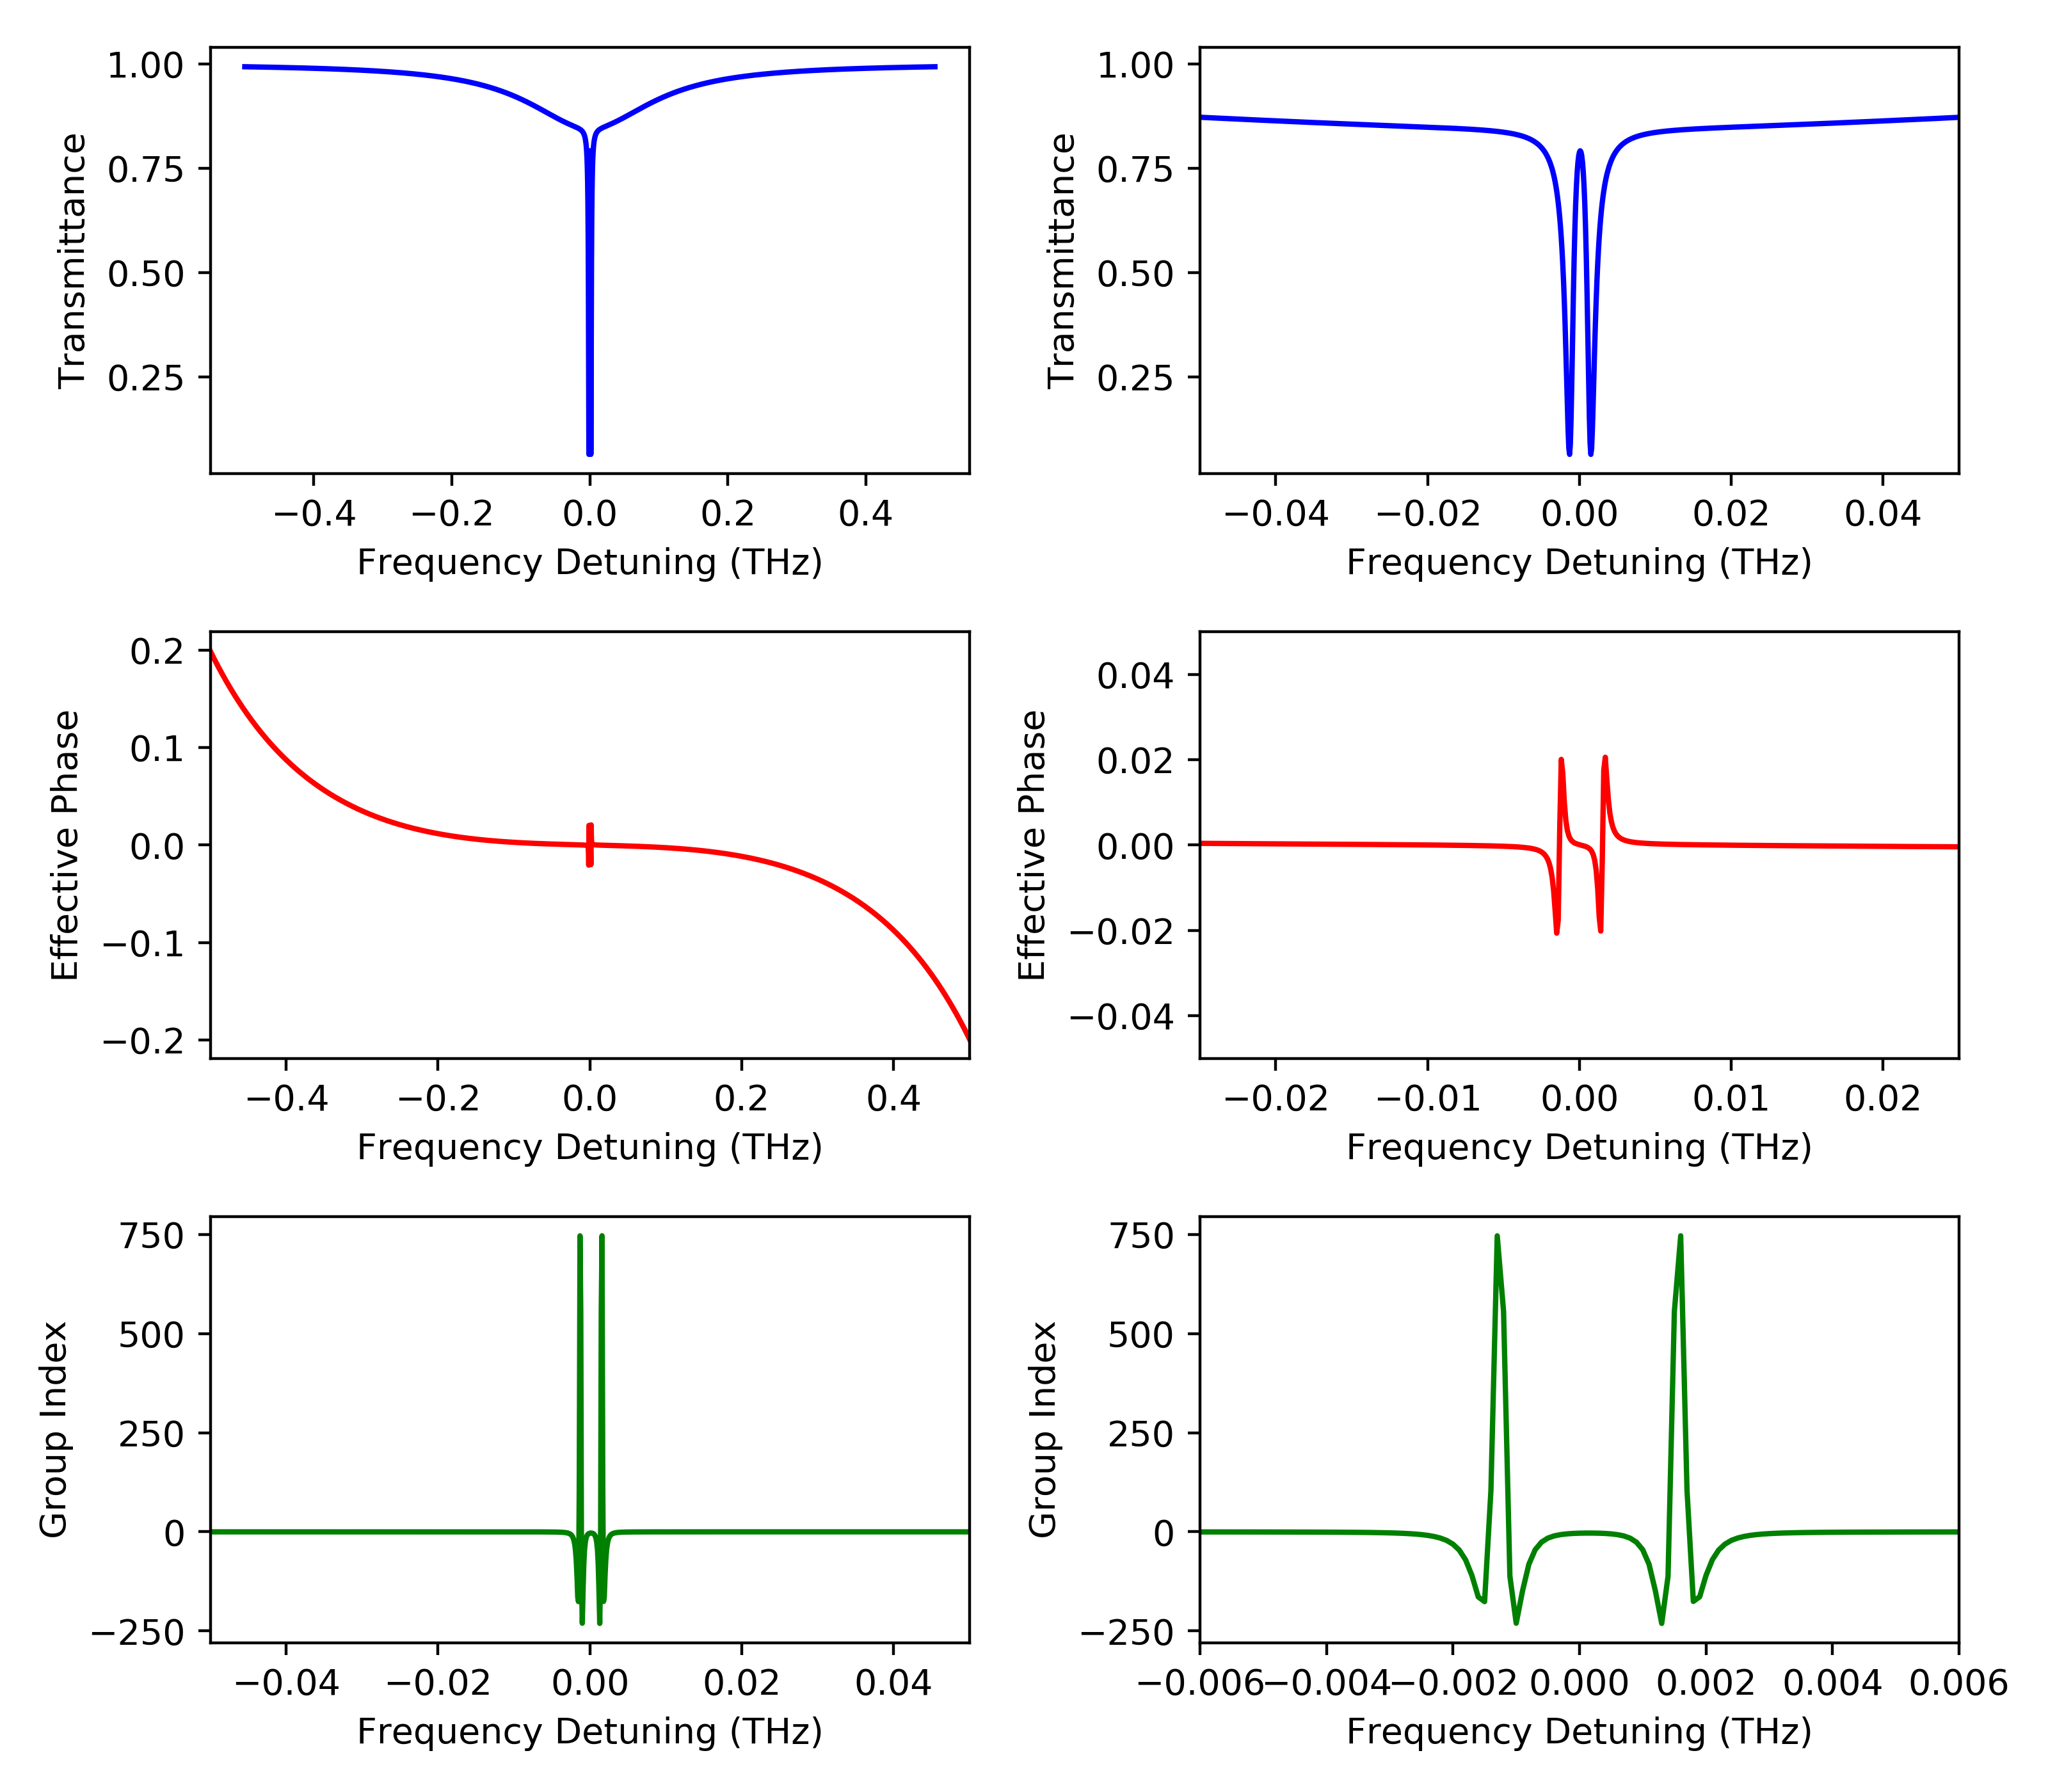
\includegraphics[width=1\textwidth]{EIT_EIA_all.eps}
\caption{CRIT observered in an CRIA transmission in three resonator system with its phase in red and group index in green.}
\end{figure}

\newpage
\subsection{CRIA inside CRIT}

After these interesting results, let us now move towards another useful transmission spectrum of our triple resonator system (see Fig. 4.3). The system parameters are given as, $r_{1} = 0.998845$, $r_{2} = 0.999988$, and $r_{3} = 0.999999$. The $\mathcal{Q}-factors$ are $1\times10^{5}, 1\times10^{6}$ and $1\times10^{7}$ for first second and third resonator respectively. This spectrum is also achieved by the same arrangement of the resonators and now we have changed the couplings once more to obtain an interesting result. 

\begin{figure}[t]
\centering
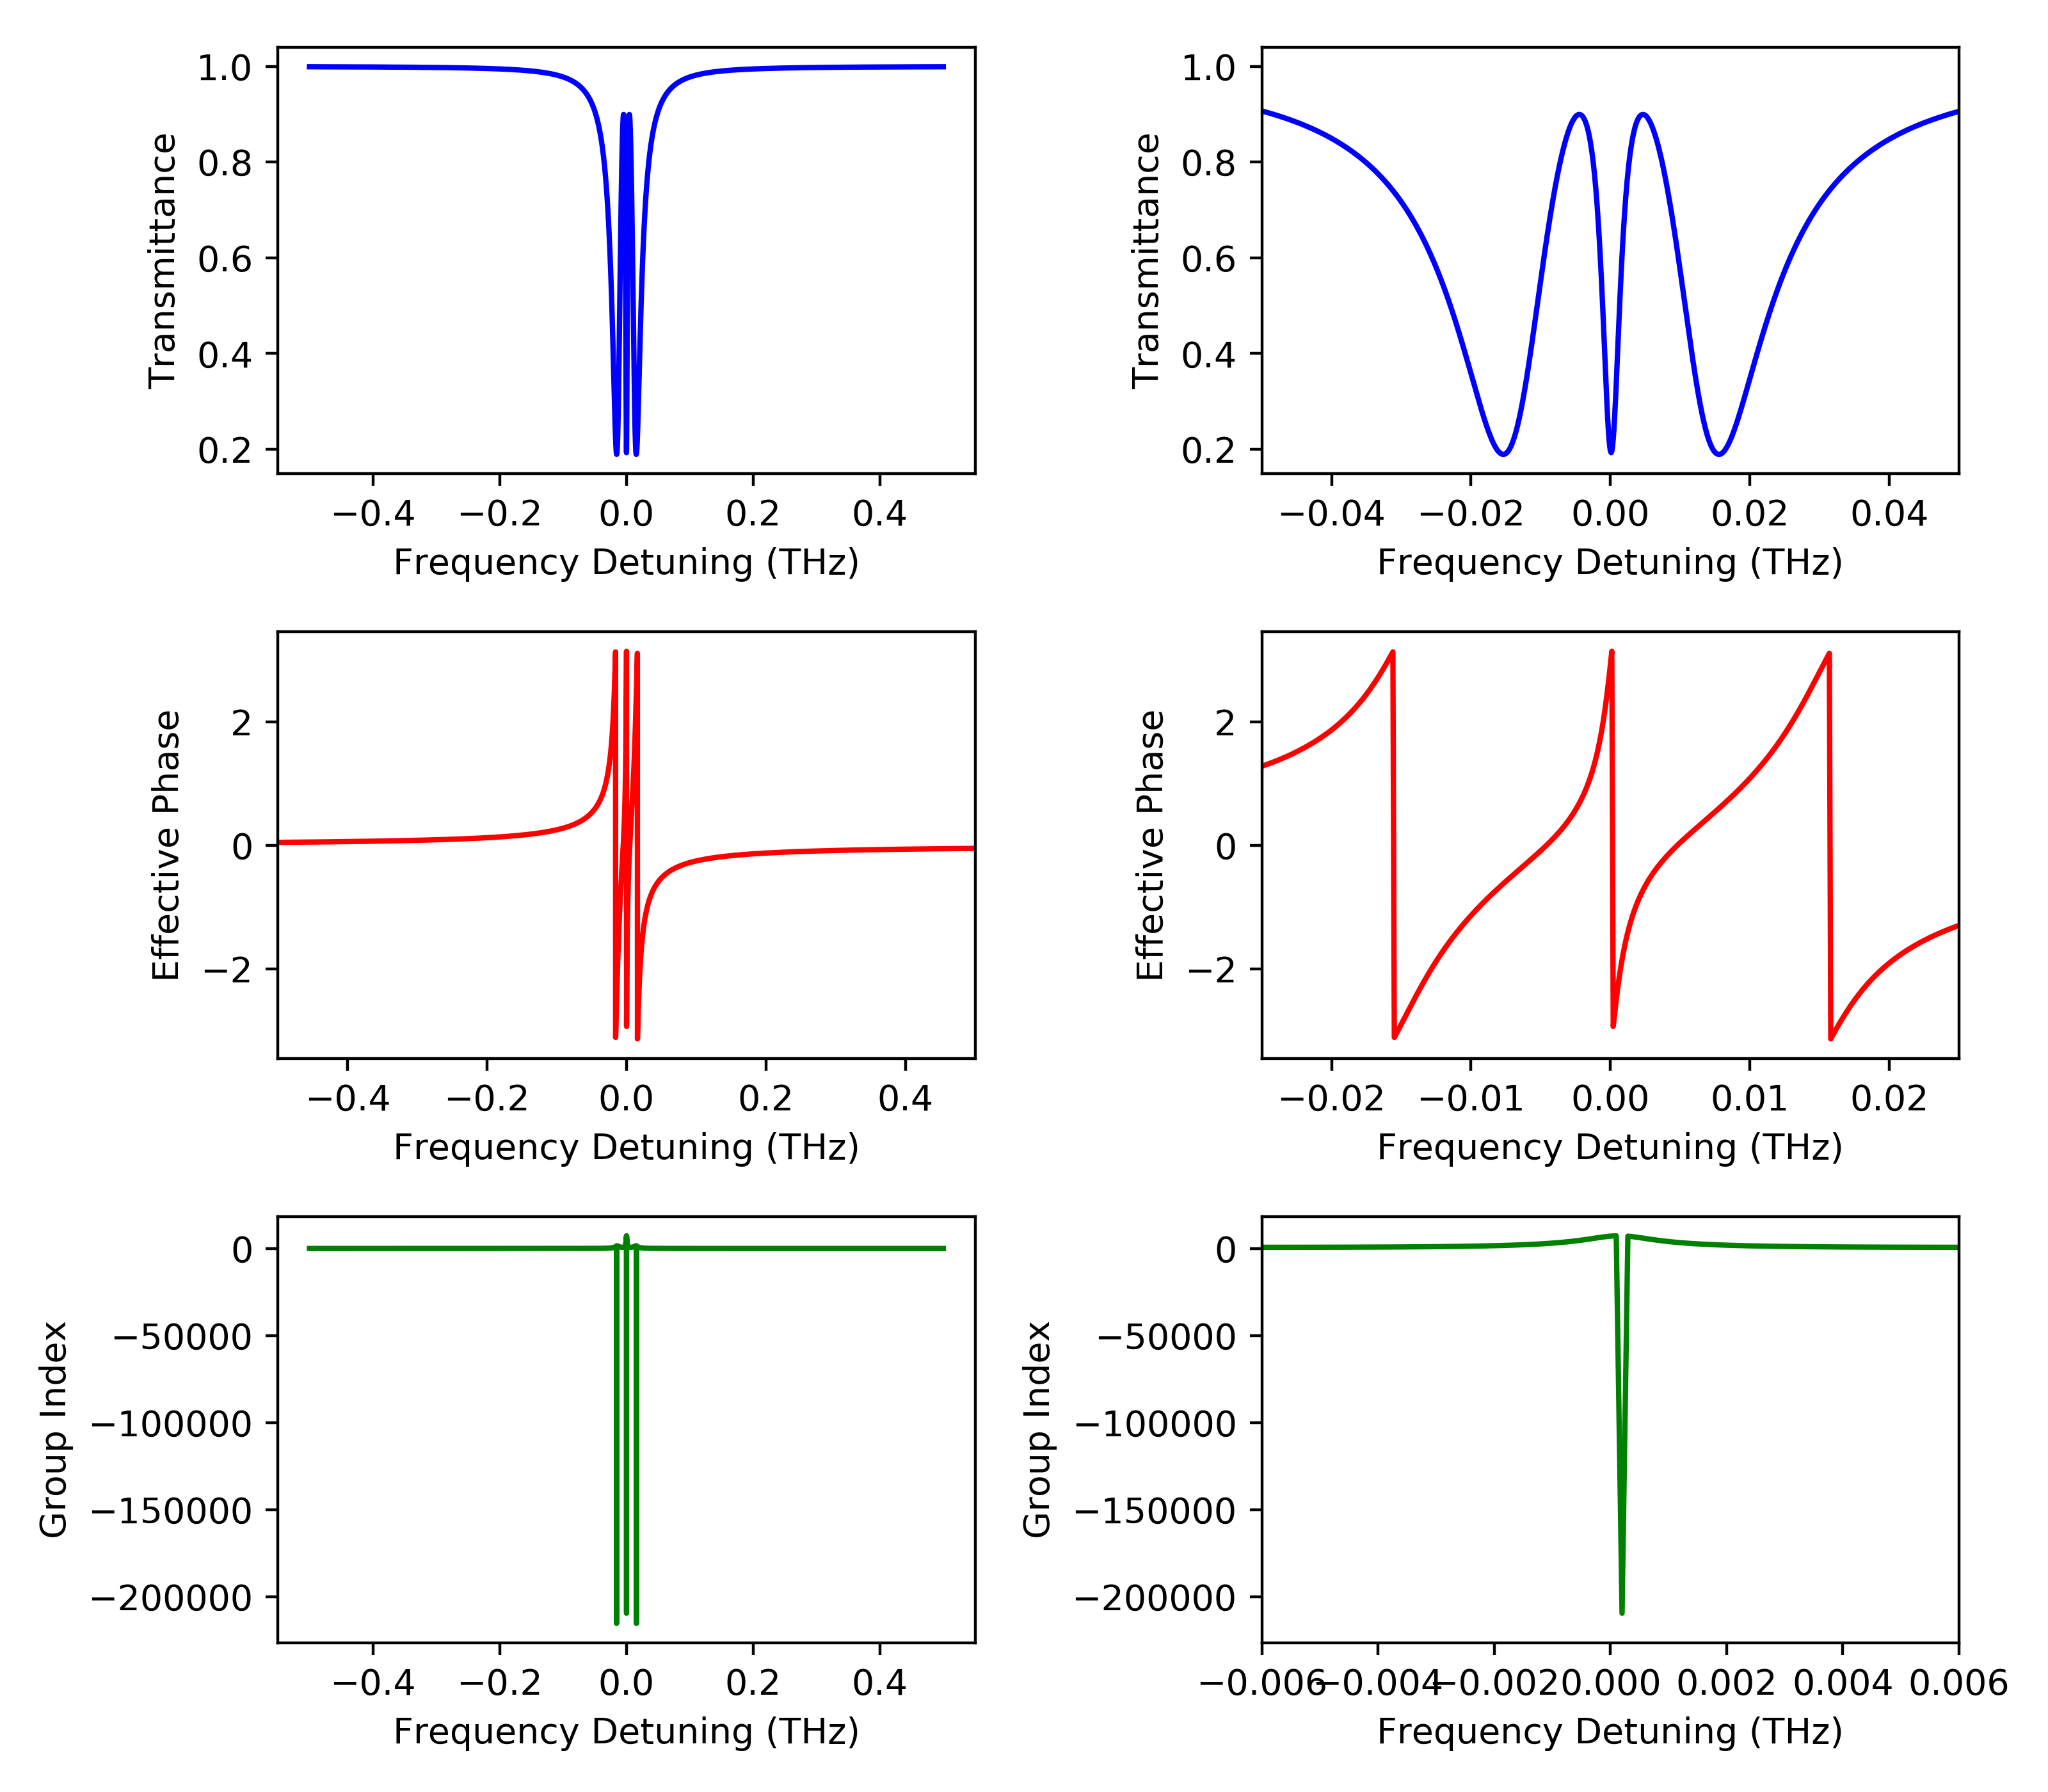
\includegraphics[width=0.90\textwidth]{EIAinEIT.eps}
\caption{CRIA observered in an CRIT transmission in three resonator system with its phase in red and group index in green.}
\end{figure}

In Fig. 4.3, we see a CRIT spectrum. When we again zoom into the transmission, we see a narrow dip on resonance. This narrow dip shows us that we actually have a CRIA resonance at the center of a CRIT resonance.

We see that the graph dips to zero almost, meaning all of the light is absorbed. This transmission dip tells us that we can filter out exactly this narrow spectrum of resonant frequencies. 
The phase of the system is shown in red and we see features of superluminous on a similar phase curve this time of quite high value. The slope of this graph is almost zero on resonance.

The group index, shown in green, also displays group index very close to zero. Although its value is $\approx -0.37$ meaning superluminal velocities of resonant frequencies. However, almost all of the resonant light circulates in the coupled resonator system and eventually dissipates. Thus this value is practically useless.


\subsection{Cascaded CRIA and CRIT in Absorption}
In Fig. 4.4, we will observe that the transmission can be a lot influenced if we were to change the coupling effects between the resonators. The system parameters are given as, $r_{1} = 0.999945$, $r_{2} = 0.999999$, and $r_{3} = 0.999999$. The $\mathcal{Q}-factors$ are $1\times10^{5}, 1\times10^{6}$ and $1\times10^{7}$ for first second and third resonator respectively. This tells us a lot about how our signal is transmitted and how much use can we achieve from the single system by changing a few of its properties. In Fig. 4.3, we change the coupling parameters in all of the resonators and have achieved a rather interesting transmission spectrum.

We can clearly see what looks like an absorption spectrum of a single resonator, has a narrow, actually CRIT peak within the broader CRIA transmission dip (zoomed on the right). This peak also has a dip on resonance due to the coupling of the third resonator. Now we observed cascaded results of CRIT within an absorption and CRIA inside that CRIT. 

The effective phase of the system, at first, also seems like that of a single resonator system but zooming into the graph tells another story. On the right, we can see three distinct features caused by coupling between the three resonators and have a negative slope on resonance. This negative slope refers that superluminal light is achieved the resonance.

The group index plot, shown in green, also displays a negative group index on resonance and positive index peaks off resonances. The negative group delay also predicts superluminal velocities of the resonant frequencies.
\newpage
\begin{figure}[h]
\centering
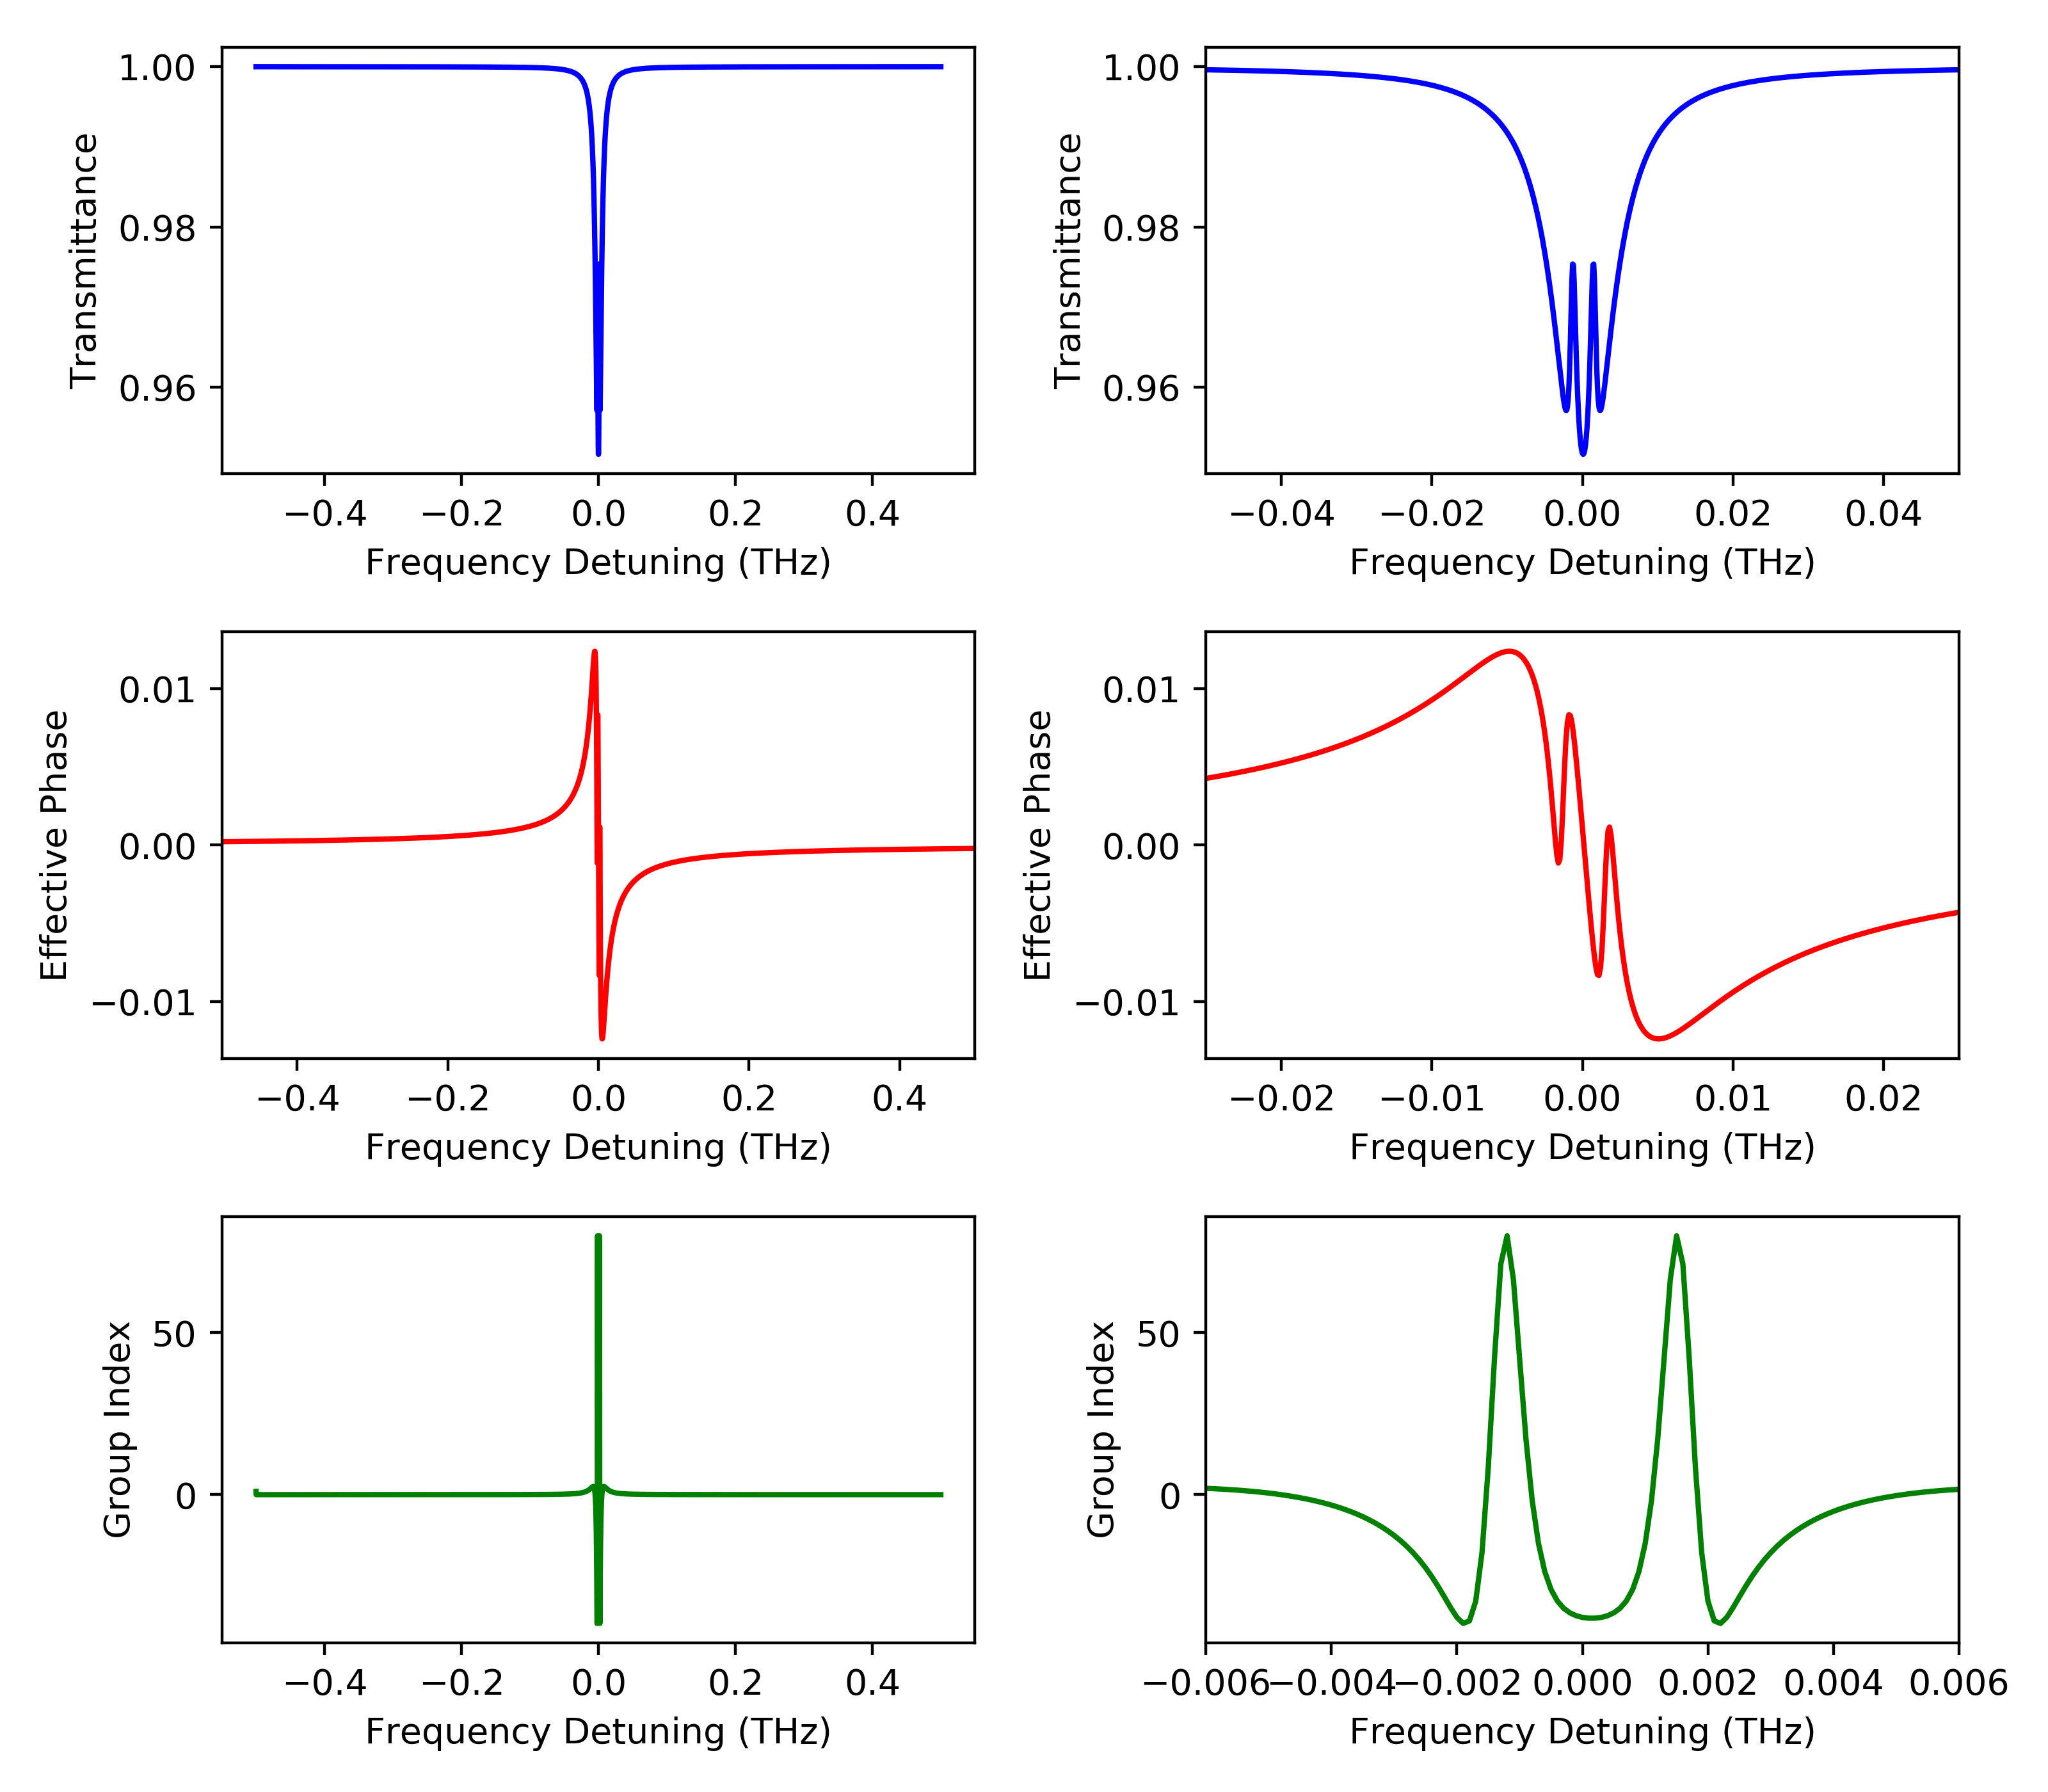
\includegraphics[width=1\textwidth]{EIT_EIA2_all.eps}
\caption{Cascaded resonance effects in the three-resonator system with its phase in red and group index in the green. Magnified views of resonances and phase are also given for clear illustration.}
\end{figure}

\subsection{Double CRIA}
We now demonstrate a double CRIA resonance (see Fig. 4.5). This means that two narrow dips are realized within a broader dip. This is in contrast to a typical CRIA where only one narrow dip is present inside a broader dip. This double EIA or CRIA is obtained by slight detuning the system and changing the coupling effects. 


\begin{figure}[t]
\centering
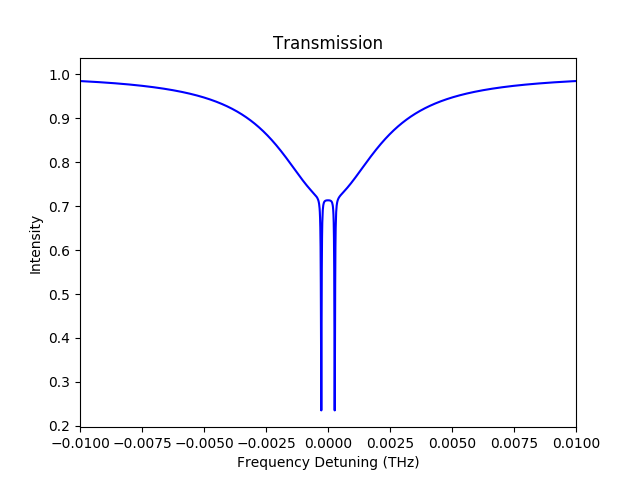
\includegraphics[scale=0.5]{2_EIA.png}
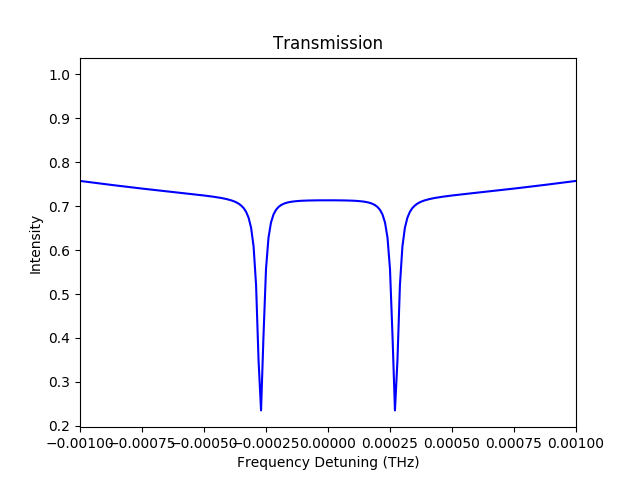
\includegraphics[scale=0.5]{2_EIAa.png}
\caption{Double transmission dips observed inside an EIA like transmission off resonant to the spectrum.}
\end{figure}

In Fig. 4.5 we can clearly see that two narrow peaks, which are caused by the two resonances of the coupled resonators, 2 and 3 respectively. And the broader dip above them is caused by the resonance of the first resonator. 


This allowed us to observe an effect which resembles the CRIA in two resonator system but this time now we have two narrow dips off resonances. This tells us that we have CRIA like properties and transmission have two narrow absorption lines but on the off-resonance. The resonant frequencies will experience very little absorption and will be mostly transmitted. 

The phase and group velocities of this case are not discussed as the purpose of this study were not to discuss the enhanced dispersion. The dispersive properties of these resonances will be similar to the ones discussed above. The true meaning is to show enhanced transmittance.


\subsection{Double CRIT}
We now demonstrate a double CRIT resonance in Fig. 4.6. This means that two narrow peaks are realized within another narrow dip on-resonance. This is in contrast to a typical CRIT where only one narrow peak is present. This double EIT or CRIT is obtained by changing the coupling effects. 

\begin{figure}[t]
\centering
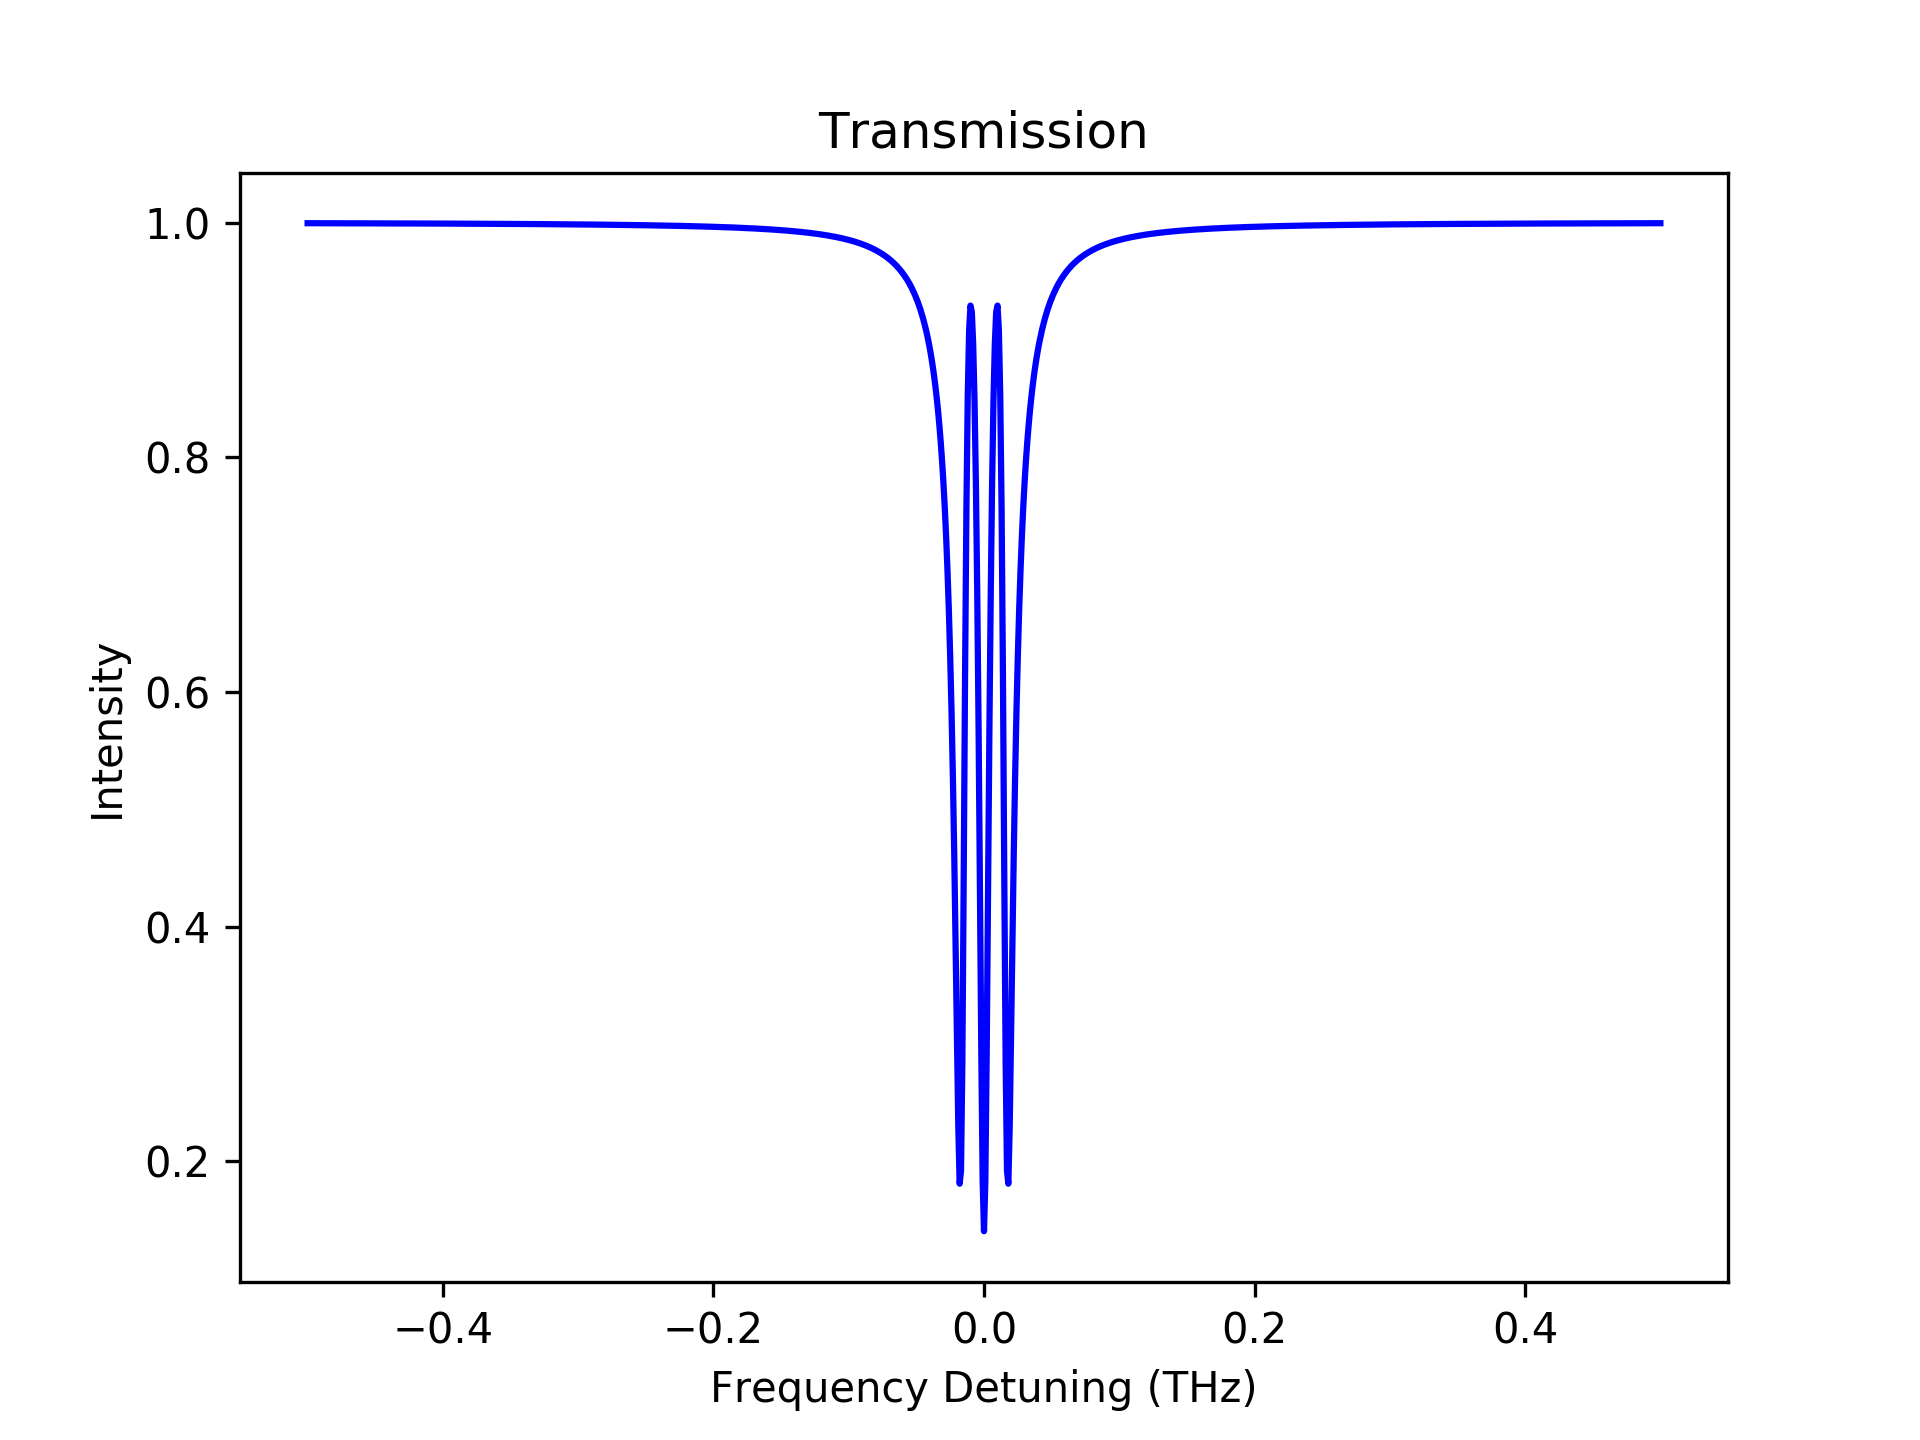
\includegraphics[scale=0.5]{double_EIT.png}
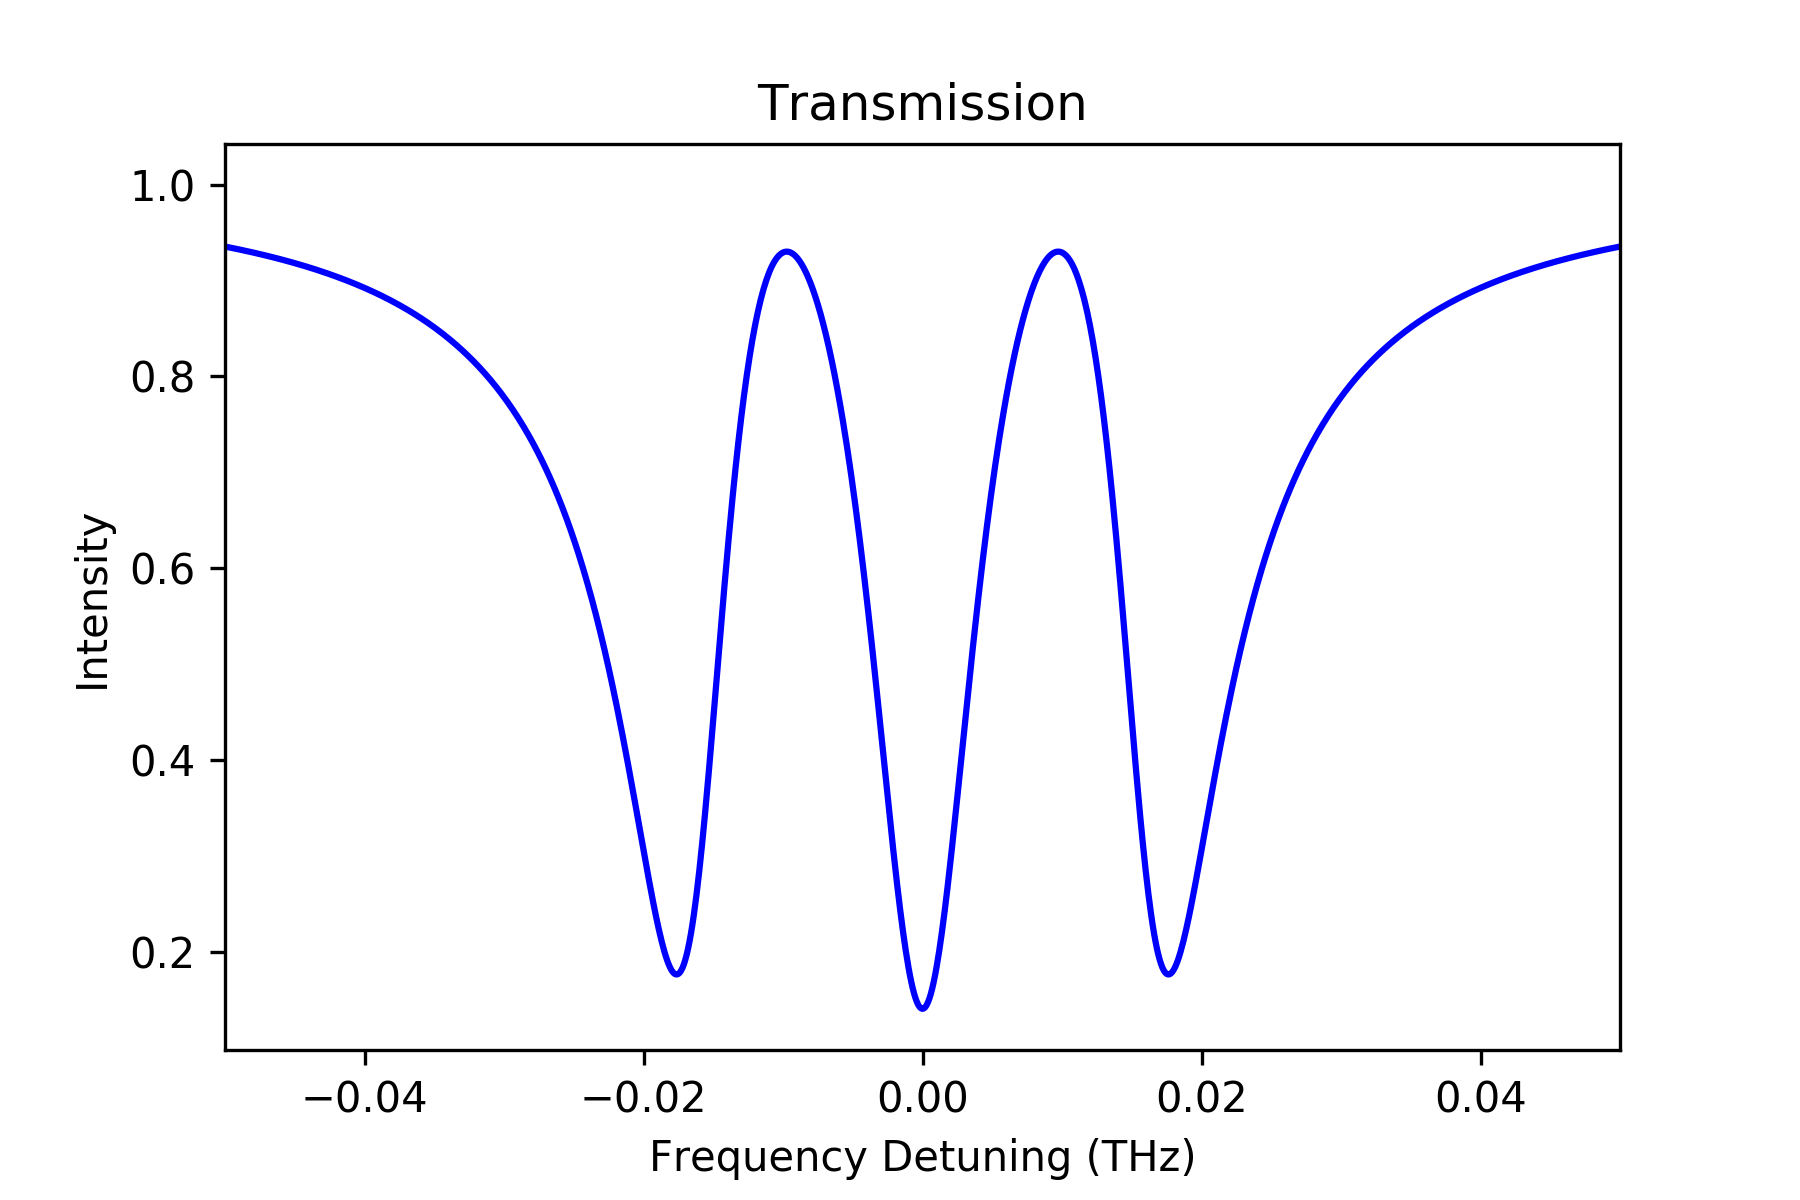
\includegraphics[scale=0.5]{double_EITa.png}
\caption{Double transmission peaks observed inside an EIT like transmission off resonant to the spectrum.}
\end{figure}


From these results, we concluded that increasing the number of resonators in the system and mutually coupling them with each other, enables us to demonstrate the versatility of the cascaded resonances. These resonances can be then utilized and achieved in practical applications to make use of them in important tasks. Optical tunability and signal filtration of specific frequencies can be achieved by using similar systems and having similar effects on them.

\newpage
\section{Discussion}
We have examined the spectral and dispersive properties of a course of three mutually coupled ring resonators. We have discovered various one of a kind cascaded resonances which show particular spectral and dispersive conduct. In view of our request, we propose new uses of coupled resonators for future quantum and optical information and communication technologies. Interacting triple cavities were previously investigated using one and two-dimensional photonic crystals for parametric oscillations [5] and group delay control [6], respectively. Furthermore, double anti-crossing behavior was recently demonstrated using triple microtoroid cavities [7]. Tunable slow and fast light in triple one-dimensional photonic crystal microcavities has also been demonstrated owing to the tuning of the resonant wavelength.

\newpage
\section*{References}
\addcontentsline{toc}{section}{References}

\paragraph{\normalfont \large $[1]$ S. H. Autler and C. H. Townes, “Stark effect in rapidly varying fields,” Phys. Rev. \textbf{100} (1955). \\ 
\\$[2]$ S. E. Harris, "Electromagnetically Induced Transparency" Physics Today, July 1997. \\
\\$[3]$ D. D. Smith, H. Chang, K. A. Fuller, A. T. Rosenberger, and R. W. Boyd, “Coupled-resonator-induced transparency,” Phys. Rev. A \textbf{69}, 063804 (2004). \\
\\$[4]$  A. Naweed, G. Farca, S. Shopova, and A. T. Rosenberger, “Induced transparency and absorption in coupled
whispering-gallery microresonators,” Phys. Rev. A \textbf{71} (2005).\\
\\$[5]$ C. Diederichs, J. Tignon, G. Dasbach, C. Ciuti, A. Lemaître, J. Bloch, P. Roussignol, and C. Delalande, “Parametric oscillation in vertical triple microcavities,” Nature \textbf{440}, 904 (2006).\\
\\$[6]$ D. O’Brien, A. Gomez-Iglesias, M. D. Settle, A. Michaeli, M. Salib, and T. F. Krauss, “Tunable optical delay using photonic crystal heterostructure nanocavities,” Appl. Phys. Rev. B \textbf{76}, 115110 (2007).\\
\\$[7]$ C. Yang,  X. Jiang Q. Hua, S. Hua, Y. Chen, and M. Xiao, “Realization of controllable photonic molecule based on three ultrahigh-Q microtoroid cavities,” Laser Photonics Rev. \textbf{11} (2007).\\
\\$[8]$ A. Naweed (to be published).}

\chapter{Conclusion}
We demonstrated gain tunable optical analogs of Electromagnetically Induced Transparency (EIT) and Electromagnetically Induced Absorption (EIA). This allowed us to precisely control superluminal and subluminal group velocities of light in a coupled ring resonator system, with a linear gain excitation and enabled reversible transitions between them. Furthermore, we observed sub and superluminal light featuring all-optical EIT resonance, which in all previous studies, based on passive coupled ring resonators, has been observed to yield only subluminal light.

 We also studied the spectral and dispersive properties of a cascade of three mutually coupled ring resonators. We have found a number of unique cascaded resonances which display distinct spectral and dispersive behavior. Based on our inquiry, we propose new applications of coupled resonators for future quantum and optical information and communication technologies.

The optimized coupled resonators demonstrate continuous variable of sub and superluminal group velocities and can be tuned owing to excitation of linear optical gain, we can observe astounding spectral characteristics. These features of coupled resonators also allow acquiring control of transmission and photon storage times inside the optical cavity. Furthermore, cascades of ring resonators additionally enhance these characteristics and exhibit unique features such as sub and superluminal at multiple wavelengths. The findings of this thesis are of great significance for the future of photonics and optical communicating systems.
\appendix
\chapter{Abrevations}

EIT Electromagnetically Induced Transparency\\
\\EIA Electromagnetically Induced Absorption\\
\\CRIT Coupled Resonator Induced Transparency\\
\\CRIA Coupled Resonator Induced Absorption\\
\\FSR Free Spectral Range\\
\\MRR Micro Ring Resonator\\
\\MZI Mach Zehnder Interferometer\\
\\FWHM Full width at half maximum\\
\\CMT Coupled Mode Theory

\chapter{Bibliography}
\paragraph{\normalfont \large $[1]$  Kaminow, I.P., Li, T., et al. Optical fiber telecommunications. 5th Edition. Academic Press, Elsevier, San Diego (2008). \\ 
\\$[2]$ A. Naweed, G. Farca, S. I. Shopova, and A. T. Rosenberger "Induced transparency and absorption in coupled whispering-gallery microresonators", Phys. Rev. A \textbf{71} (2005)\\
\\$[3]$ B. Peng1, S. K. Ozdemir, W. Chen, F. Nori, L. Yang "What is and what is not electromagnetically induced transparency in whispering-gallery microcavities", Nature. Comm. (2014). \\
\\$[4]$ John E. Heebner, Ph.D. Thesis, "Nonlinear Optical Whispering Gallery Microresonators for Photonics", (2003)  \\
\\$[5]$ K. J. Vahala, “Optical microcavities,” Nature \textbf{424} (2003).\\
\\$[6]$ L. Maleki, A. B. Matsko, A. A. Savchenkov, and V. S. Ilchenko, “Tunable delay line with interacting
whispering-gallery-mode resonators,” Opt. Lett. 29(6), 626–628 (2004).\\
\\$[7]$ A. Naweed, D. Goldberg, and V. M. Menon, “All-optical electromagnetically induced transparency using
coupled one-dimensional microcavities,” Opt. Express 22, 18818–18823 (2014).\\
\\$[8]$ M. Borselli, T. Johnson, and O. Painter, “Beyond the Rayleigh scattering limit in high-Q silicon microdisks:
theory and experiment,” Opt. Express 13(5), 1515–1530 (2005).\\
\\$[9]$ Kobrinsky, M. J., Block, B.A., et al. On-chip optical interconnects. Intel Technol. J. \textbf{8}, 129 (2004).\\
\\$[10]$ Barwicz, T., Byun, H., et al. Silicon photonics for compact, energy-efficient interconnects. J. Opt. Networking \textbf{6}, 63 (2007)\\
\\$[11]$ Ishikawa, H. Ultrafast all-optical signal processing devices. John Wiley and Sons, New Jersey (2008). \\
\\$[12]$ Xia, F., Sekaric, L., et al. Ultracompact optical buffers on a silicon chip. Nature \textbf{1}, 65–71
(2007).\\
\\$[13]$ Landobasa, Y.M., Chin, M.K. Optical buffer with higher delay-bandwidth product in a tworing system. Opt. Express \textbf{16}, 1796–1807 (2008).
\\$[14]$ Fabry, C., Pérot, A. Théorie et applications d’une nouvelle méthode de spectroscopie interférentielle. Ann. Chim. Phys. \textbf{16}, 115 (1899).\\
\\$[15]$ M. Bayindir, S. Tanriseven, A. Aydinli, and E. Ozbay, “Strong enhancement of spontaneous emission in
amorphous-silicon-nitride photonic crystal based coupled-microcavity structures,” Appl. Phys., A Mater. Sci.
Process. \textbf{73}(1), 125–127 (2001)\\
\\$[16]$ M. Bayindir, S. Tanriseven, A. Aydinli, and E. Ozbay, “Strong enhancement of spontaneous emission in
amorphous-silicon-nitride photonic crystal based coupled-microcavity structures,” Appl. Phys., A Mater. Sci.
Process. \textbf{73}(1), 125–127 (2001).\\
\\$[17]$ A. J. Campillo, J. D. Eversole, and H.-B. Lin, “Cavity quantum electrodynamic enhancement of stimulated
emission in microdroplets,” Phys. Rev. Lett. \textbf{67}(4), 437–440 (1991).\\
\\$[18]$ D. Gerace, H. E. Türeci, A. Imamoglu, V. Giovannetti, and R. Fazio, “The quantum-optical Josephson
interferometer,” Nat. Phys. \textbf{5}(4), 281–284 (2009).\\
\\$[19]$  C. Diederichs, J. Tignon, G. Dasbach, C. Ciuti, A. Lemaître, J. Bloch, P. Roussignol, and C. Delalande,
“Parametric oscillation in vertical triple microcavities,” Nature \textbf{440}(7086), 904–907 (2006).\\
\\$[20]$ Q. Xu, S. Sandhu, M. L. Povinelli, J. Shakya, S. Fan, and M. Lipson, “Experimental realization of an on-chip alloptical analogue to electromagnetically induced transparency,” Phys. Rev. Lett. \textbf{96}(12), 123901 (2006).}

\paragraph{\normalfont \large $[21]$ J. Heebner, R. Grover, T. Ibrahim "Optical Microresonators, Theory, Fabrication, and Applications", Springer Science+Business Media (2008)\\
\\ $[22]$ K. Totsuka and M. Tomita "Dynamics of fast and slow pulse propagation through a microsphere–optical-fiber system", Phy. Rev. E \textbf{75} (2007)\\
\\ $[23]$ D. D. Smith, H. Chang, K. A. Fuller, A. T. Rosenberger, and R. W. Boyd, “Coupled-resonator-induced
transparency,” Phys. Rev. A \textbf{69}, 063804 (2004)\\
\\ $[24]$ A. J. Campillo, J. D. Eversole, and H.-B. Lin, “Cavity quantum electrodynamic enhancement of stimulated
emission in microdroplets,” Phys. Rev. Lett. \textbf{67}(4), 437–440 (1991).\\
\\ $[25]$ C. G. B. Garrett, and D. E. McCumber,  "Propagation of a Gaussian light pulse through an anomalous dispersion medium." Phys. Rev. A \textbf{1}, 305 (1970).\\
\\ $[26]$ Chu, S. and Wong, S. Linear pulse propagation in an absorbing medium. Phys. Rev. Lett. \textbf{48}, 738
(1982).\\
\\ $[27]$ Chiao, R. Y. Superluminal (but causal) propagation of wave packets in transparent media with inverted atomic populations. Phys. Rev. A \textbf{48}, R34 (1993).\\
\\ $[28]$ Bolda, E., Garrison, J. C. and Chiao, R. Y. Optical pulse propagation at negative group velocities due to a nearby gain line. Phys. Rev. A \textbf{49}, 2938 (1994).\\
\\ $[29]$ R.W. Boyd and D. Gauthier "Controlling the Velocity of Light Pulses", Science \textbf{326} (2009)\\
\\ $[30]$ L. J. Wang, A. Kuzmich and A. Dogariu "Gain-assisted superluminal light propagation", Nature \textbf{406} (2000)\\
\\ $[31]$  S. Y. Hu, E. R. Hegblom, and L. A. Coldren, “Coupled-cavity resonant-photodetectors for high-performance
wavelength demultiplexing applications,” Appl. Phys. Lett. \textbf{71}(2), 178–180 (1997).\\
\\ $[32]$  Z. Shi, R. W. Boyd, D. J. Gauthier, C. C. Dudley, “Enhancing the spectral sensitivity of interferometers
using slow-light media” Opt. Let. \textbf{32}, 8 (2007).\\
\\ $[33]$  M. Salit, G. S. Pati, K. Salit and M. S. Shahriar “Fast-light for astrophysics: super-sensitive gyroscopes and gravitational wave detectors” Journal of Modern Optics \textbf{54}, 16 (2007).\\
\\ $[34]$\,  Hecht, Jeff. The Laser Guidebook: Second Edition. McGraw-Hill, 1992. (Chapter 18-21).\\
\\ $[35]$  F. J. Duarte and L. W. Hillman (Eds.), Dye Laser Principles (Academic, New York, 1990).\\
\\ $[36]$ A. Naweed, "Photonic coherence effects from dual-waveguide coupled pair of co-resonant microring resonators", Opt. Exp. \textbf{23} (2015).\\
\\ $[37]$ Hau, L. V., Harris, S. E., Dutton, Z. and Behroozi, C. H. Light speed reduction to 17 meters per second in
an untracold atomic gas. Nature \textbf{397}, 594 (1999).\\
\\ $[38]$  Kash, M. M. et al. Ultraslow group velocity and enhanced nonlinear optical effects in a coherently
driven hot atomic gas. Phys. Rev. Lett. \textbf{82}, 5229 (1999).\\
\\ $[39]$ Budker, D., Kimball, D. F., Rochester, S. M. and Yashchuk, V. V. Nonlinear magneto-optics and reduced
group velocity of light in atomic vapor with slow ground state relaxation. Phys. Rev. Lett. \textbf{83}, 1767 (1999).\\
\\ $[40]$ Einstein, A., Lorentz, H. A., Minkowski, H. and Weyl, H. The Principle of Relativity, Collected Papers
(Dover, New York, 1952).}


\paragraph{\normalfont \large $[41]$ S. H. Autler and C. H. Townes, “Stark effect in rapidly varying fields,” Phys. Rev. \textbf{100} (1955) \\ 
\\$[42]$ S. E. Harris, "Electromagnetically Induced Transparency" Physics Today, July 1997 \\
\\$[43]$ X. Yang, M. Yu, D.-L. Kwong, and C. W. Wong, “All-optical analog to electromagnetically induced
transparency in multiple coupled photonic crystal cavities,” Phys. Rev. Lett. \textbf{102}(17), 173902 (2009). \\
\\$[44]$  O. Deparis and O. El Daif, “Optimization of slow light one-dimensional Bragg structures for photocurrent
enhancement in solar cells,” Opt. Lett. \textbf{37}(20), 4230–4232 (2012).\\
\\ $[45]$ B. Peng1, S. K. Ozdemir, W. Chen, F. Nori, L. Yang "What is and what is not electromagnetically induced transparency in whispering-gallery microcavities", Nature. Comm. (2014).\\
\\ $[46]$ Y.C. Liu, B.B. Li, and Y.F. Xiao "Electromagnetically induced transparency in optical microcavities", nanoph-2016-0168, (2017).\\
\\ $[47]$ S. Zhu, L. Shi, S. Yuan, R. Ma, X. Zhang and X. Fan, "All-optical controllable electromagnetically induced transparency in coupled silica microbottle cavities", nanoph-2018-0111 (2018).\\
\\ $[48]$ J. F. McMillan, X. Yang, N. C. Panoiu, R. M. Osgood, and C. W. Wong, “Enhanced stimulated Raman scattering
in slow-light photonic crystal waveguides,” Opt. Lett. \textbf{31}(9), 1235–1237 (2006).\\
\\ $[49]$ K. Totsuka, N. Kobayashi, and M. Tomita, “Slow light in coupled-resonator-induced transparency,” Phys. Rev.
Lett. \textbf{98}(21), 213904 (2007).\\
\\ $[50]$ A. Naweed (to be published)}

\paragraph{\normalfont \large $[51]$ S. H. Autler and C. H. Townes, “Stark effect in rapidly varying fields,” Phys. Rev. \textbf{100} (1955) \\ 
\\$[52]$  N. Miladinovic, F. Hasan, N. Chisholm, I. E. Linnington, E. A. Hinds, and D. H. J. O’Dell, “Adiabatic transfer of light in a double cavity and the optical Landau-Zener problem,” Phys. Rev. A \textbf{84}(4), 043822 (2011).\\
\\$[53]$ X. Yang, C. Husko, C. W. Wong, M. Yu, and D.-L. Kwong, “Observation of femtojoule optical bistability
involving Fano resonances in high-Q/V silicon photonic crystal nanocavities,” Appl. Phys. Lett. \textbf{91}(5), 051113
(2007).\\
\\$[54]$  V. M. Menon, W. Tong, and S. R. Forrest, “Control of quality factor and critical coupling in microring resonators
through integration of a semiconductor optical amplifier,” IEEE Photon. Technol. Lett. \textbf{16}(5), 1343–1345 (2004).\\
\\$[55]$ C. Diederichs, J. Tignon, G. Dasbach, C. Ciuti, A. Lemaître, J. Bloch, P. Roussignol, and C. Delalande,“Parametric oscillation in vertical triple microcavities,” Nature \textbf{440}(7086), 904–907 (2006).\\
\\$[56]$ D. O’Brien, A. Gomez-Iglesias, M. D. Settle, A. Michaeli, M. Salib, and T. F. Krauss, “Tunable optical delay using photonic crystal heterostructure nanocavities ,” Appl. Phys. Rev. B \textbf{76}, 115110 (2007).\\
\\$[57]$ C. Yang,  X. Jiang Q. Hua, S. Hua, Y. Chen, and M. Xiao, “Realization of controllable photonic molecule based on three ultrahigh-Q microtoroid cavities,” Laser Photonics Rev., 2017, \textbf{11},\\
\\$[58]$ X. Yang, M. Yu, D.-L. Kwong, and C. W. Wong, “All-optical analog to electromagnetically induced
transparency in multiple coupled photonic crystal cavities,” Phys. Rev. Lett. \textbf{102}(17), 173902 (2009).\\
\\$[59]$ D. Cui, C. Xie, Y. Liu, Y. Li, L. Wei, Y. Wang, J. Liu, and C. Xue, “Experimental demonstration of inducedtransparency based on a novel resonator system,” Opt. Commun. 324, 296–300 (2014).\\
\\$[60]$ A. Naweed (private communications).}

\end{document}